\documentclass[12pt,a4paper]{article}

\usepackage[a4paper,margin=1in]{geometry}
\setlength{\headheight}{14.5pt}
\addtolength{\topmargin}{-2.5pt}
\usepackage{graphicx}
\graphicspath{{../output_plots/}}
\usepackage{booktabs}
\usepackage{amsmath,amssymb}
\usepackage{float}
\usepackage{xurl}
\usepackage{hyperref}
\usepackage{xcolor}
\usepackage{listings}
\usepackage{enumitem}
\usepackage{fancyhdr}
\usepackage{longtable}

\hypersetup{colorlinks=true,linkcolor=blue,urlcolor=blue}

\pagestyle{fancy}
\fancyhf{}
\lhead{ICS1512}
\rhead{Machine Learning Algorithms Laboratory}
\cfoot{\thepage}

\lstset{
language=Python,
basicstyle=\ttfamily\small,
numbers=left,
frame=single,
breaklines=true,
showstringspaces=false
}

\begin{document}

\noindent
\begin{tabular}{|p{3.8cm}|p{11.2cm}|}
\hline
\textbf{Experiment No.} & 9 \\ \hline
\textbf{Experiment Title} & Perceptron vs Multilayer Perceptron (A/B Experiment) with Hyperparameter Tuning\footnotemark \\ \hline
\textbf{Student Name} & Danusu K \\ \hline
\textbf{Register Number} & 3122247001013 \\ \hline
\textbf{Faculty} & Dr. Poreddy Ajay Kumar Reddy \\ \hline
\textbf{Submission Date} & \today \\ \hline
\end{tabular}
\footnotetext{\textbf{GitHub Repository: }\url{https://github.com/Danush-k/Machine-Learning}}

\section{Objective}
\begin{itemize}
\item To implement \textbf{Model A: Single-Layer Perceptron Learning Algorithm (PLA)} from scratch (step activation, classical weight-update rule) as a multiclass One-vs-Rest classifier.
\item To implement \textbf{Model B: Multilayer Perceptron (MLP)} with hidden layers and non-linear activations, trained via backpropagation.
\item To select and justify MLP hyperparameters — activation function, cost function, optimizer, learning rate, hidden-layer architecture, and batch size — through systematic staged hyperparameter tuning.
\item To rigorously compare PLA and tuned MLP using Accuracy, Precision, Recall, F1-score, confusion matrices, micro/macro-average ROC curves, and training convergence curves, on the \textbf{English Handwritten Characters} dataset (62 classes: 0--9, A--Z, a--z).
\end{itemize}

\section{Problem Statement}
Handwritten character recognition is a classical, genuinely non-linear pattern-recognition problem: strokes forming visually similar characters (e.g., '0'/'O', 'l'/'I'/'1') cannot be separated by simple linear decision boundaries in raw pixel space. This experiment uses a small, balanced 62-class handwritten character dataset (3,410 images, 55 per class) to directly contrast a purely linear classifier (the Perceptron) against a non-linear, hidden-layer network (the MLP), quantifying exactly how much representational and optimization power is gained by moving from a single trainable linear layer to a tuned, multi-parameter non-linear architecture — while also confronting the practical challenges (dying activations, optimizer divergence, overfitting with limited per-class samples) that arise when tuning a neural network on a small dataset.

\section{Theoretical Background}

\subsection{Perceptron Learning Algorithm (PLA)}
The perceptron computes a linear decision function using a step activation:
\begin{equation}
\hat{y} = \begin{cases} 1 & \text{if } \mathbf{w}\cdot\mathbf{x} + b \ge 0 \\ 0 & \text{otherwise} \end{cases}
\end{equation}
and updates its weights using the classical rule:
\begin{equation}
\mathbf{w}_{t+1} = \mathbf{w}_t + \eta(y - \hat{y})\,\mathbf{x}
\end{equation}
For a $K$-class problem, PLA is extended via the \textbf{One-vs-Rest (OvR)} scheme: $K$ independent binary perceptrons $\{\mathbf{w}_c\}_{c=1}^{K}$ are trained simultaneously, each learning to separate class $c$ from all others; the predicted class is $\arg\max_c (\mathbf{w}_c \cdot \mathbf{x})$. By the Perceptron Convergence Theorem, this update rule is guaranteed to converge \textit{only if the classes are linearly separable}; otherwise, the algorithm oscillates indefinitely without ever finding a stable separating hyperplane.

\subsection{Multilayer Perceptron (MLP)}
An MLP stacks one or more hidden layers of the form $\mathbf{h}^{(l)} = \phi(\mathbf{W}^{(l)}\mathbf{h}^{(l-1)} + \mathbf{b}^{(l)})$ between the input and a softmax output layer, where $\phi$ is a non-linear activation (ReLU, Sigmoid/Logistic, or Tanh). Parameters are trained via \textbf{backpropagation} to minimize the multiclass cross-entropy loss:
\begin{equation}
\mathcal{L} = -\frac{1}{N}\sum_{i=1}^{N}\sum_{c=1}^{K} y_{i,c}\log(\hat{y}_{i,c})
\end{equation}
using gradient-based optimizers such as plain Stochastic Gradient Descent (SGD) or Adam (adaptive per-parameter moment estimation). Unlike PLA, the composition of non-linear hidden layers allows the MLP to approximate arbitrary non-linear decision boundaries (Universal Approximation Theorem), at the cost of a substantially larger, non-convex hyperparameter and optimization search space.

\section{Dataset Description \& Preprocessing}
\begin{longtable}{|p{5.5cm}|p{8.5cm}|}
\hline
\textbf{Attribute} & \textbf{Specification} \\ \hline
\endhead
Dataset Name & English Handwritten Characters Dataset \\ \hline
Total Samples & 3,410 images (exactly 55 per class, perfectly balanced) \\ \hline
Number of Classes & 62 (digits 0--9, uppercase A--Z, lowercase a--z) \\ \hline
Raw Image Format & 1200$\times$900 RGB, black ink on white background \\ \hline
Preprocessing & Grayscale conversion $\to$ resize to $28\times28$ (Lanczos) $\to$ flatten to 784-d $\to$ normalize to $[0,1]$ \\ \hline
Label Encoding & \texttt{LabelEncoder} (62 classes $\to$ integers 0--61) \\ \hline
Train-Test Split & 80\% train (2,728 images, $\sim$44/class) / 20\% test (682 images, $\sim$11/class), stratified, seed=42 \\ \hline
\end{longtable}

\begin{figure}[H]
\centering
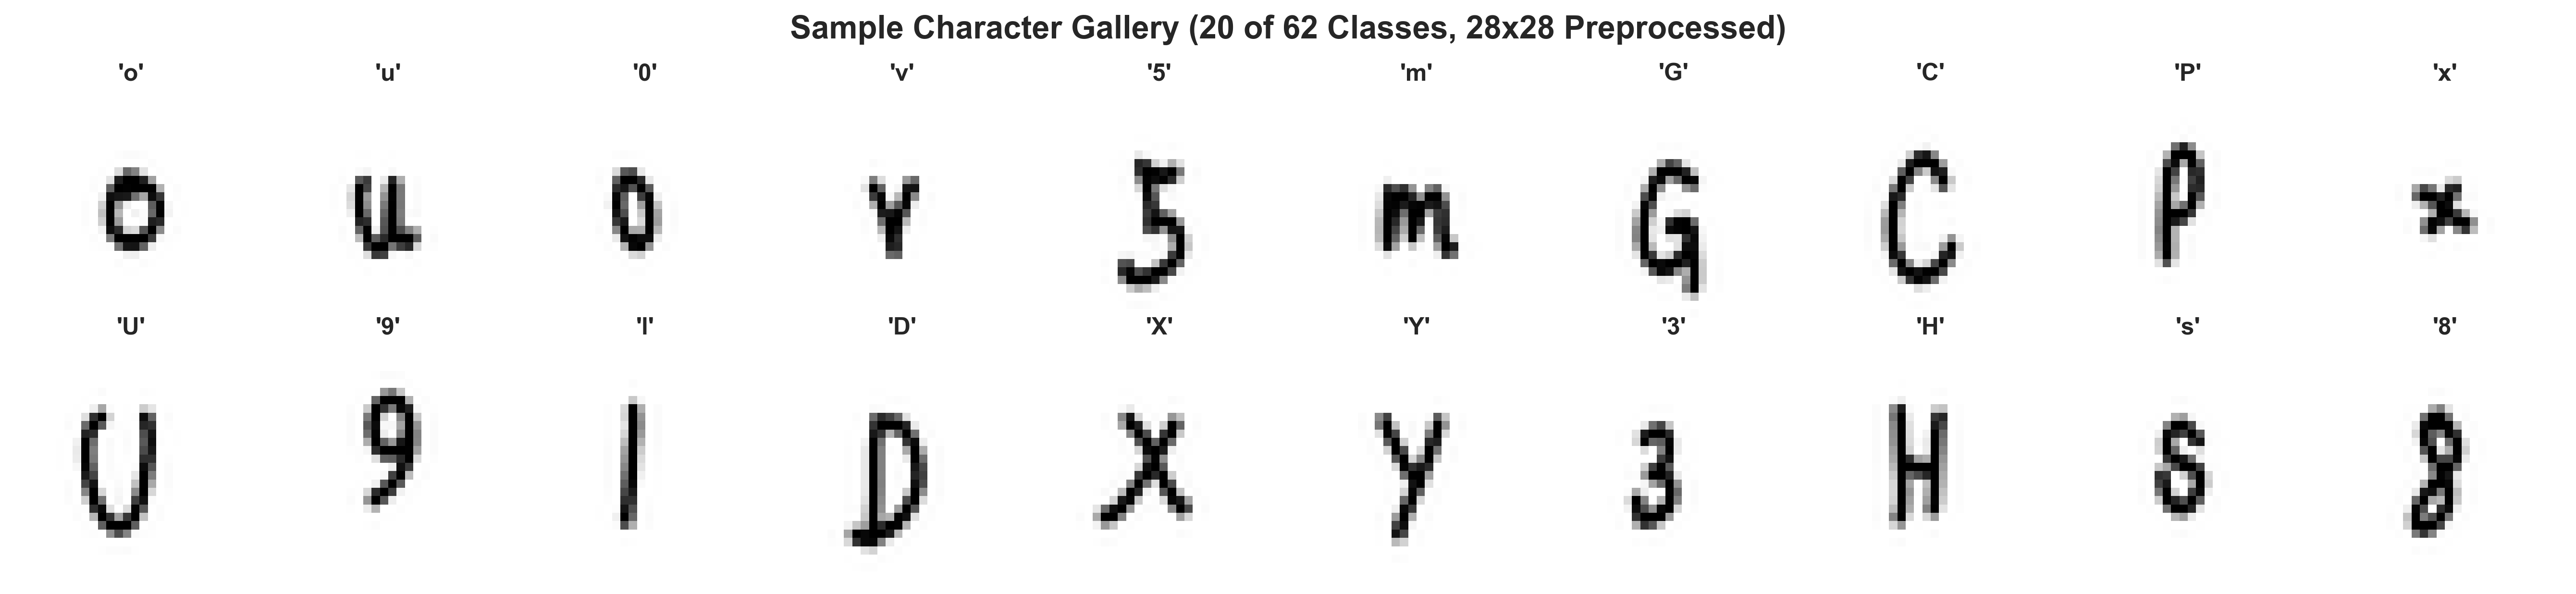
\includegraphics[width=0.98\linewidth]{01_sample_character_gallery.png}
\caption{Sample Character Gallery — 20 of 62 Classes, Preprocessed to 28$\times$28 Grayscale.}
\end{figure}

\section{Model A: PLA Implementation \& Results}

\subsection{Training Convergence}
Table~\ref{tab:pla_convergence} and Figure~\ref{fig:pla_conv} show PLA's train/test accuracy and misclassification count across 60 training epochs.

\begin{table}[H]
\centering
\caption{PLA Training Convergence (Selected Epochs)}
\label{tab:pla_convergence}
\begin{tabular}{ccccc}
\toprule
\textbf{Epoch} & \textbf{Train Acc.} & \textbf{Test Acc.} & \textbf{Weight Updates} \\
\midrule
1 & 3.70\% & 3.81\% & 2,689 \\
10 & 14.81\% & 11.29\% & 2,544 \\
20 & 24.71\% & 14.96\% & 2,427 \\
30 & 33.54\% & 19.50\% & 2,369 \\
40 & 28.37\% & 15.40\% & 2,325 \\
50 & 28.37\% & 17.60\% & 2,283 \\
\textbf{60 (Final)} & \textbf{37.72\%} & \textbf{18.62\%} & 2,253 \\
\bottomrule
\end{tabular}
\end{table}

\noindent
\textbf{Observation:} PLA never converges to a stable solution — accuracy and misclassification counts oscillate rather than monotonically improving, because the 62-class handwritten-character feature space is not linearly separable.

\begin{figure}[H]
\centering
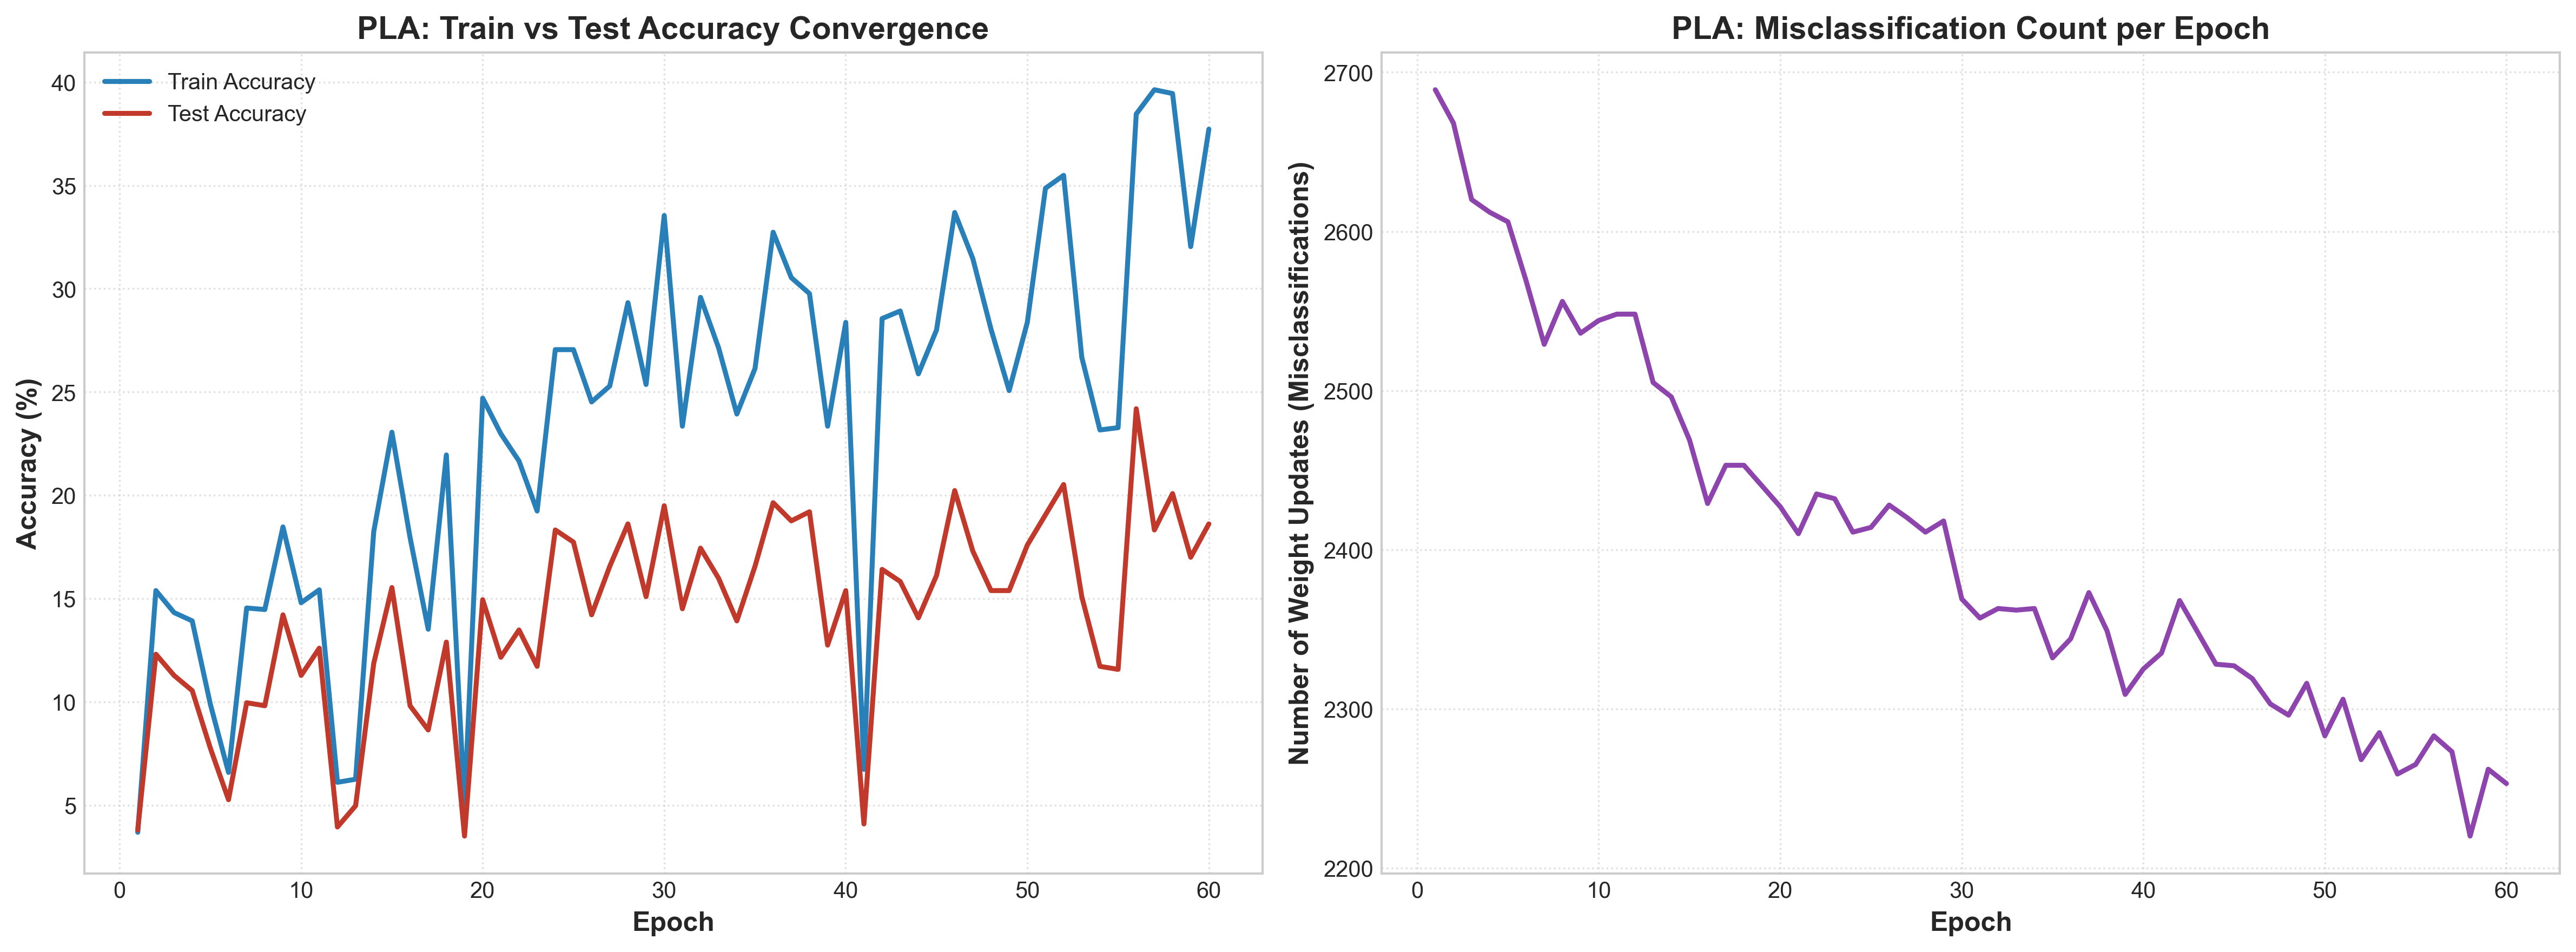
\includegraphics[width=0.98\linewidth]{03_pla_training_convergence.png}
\caption{PLA Train vs Test Accuracy Convergence, and Misclassification Count per Epoch.}
\label{fig:pla_conv}
\end{figure}

\subsection{Learning-Rate Sensitivity}
\begin{table}[H]
\centering
\caption{PLA Learning-Rate ($\eta$) Sensitivity (20 Epochs)}
\begin{tabular}{cc}
\toprule
\textbf{Learning Rate ($\eta$)} & \textbf{Final Test Accuracy} \\
\midrule
0.001 & 14.96\% \\
0.01 & 14.96\% \\
0.1 & 14.96\% \\
1.0 & 14.96\% \\
\bottomrule
\end{tabular}
\end{table}

\noindent
\textbf{Observation:} Accuracy is exactly identical across all four learning rates — a direct empirical confirmation that, with zero-initialized weights, the perceptron's sign-based decision rule is invariant to uniform positive rescaling of $\eta$.

\begin{figure}[H]
\centering
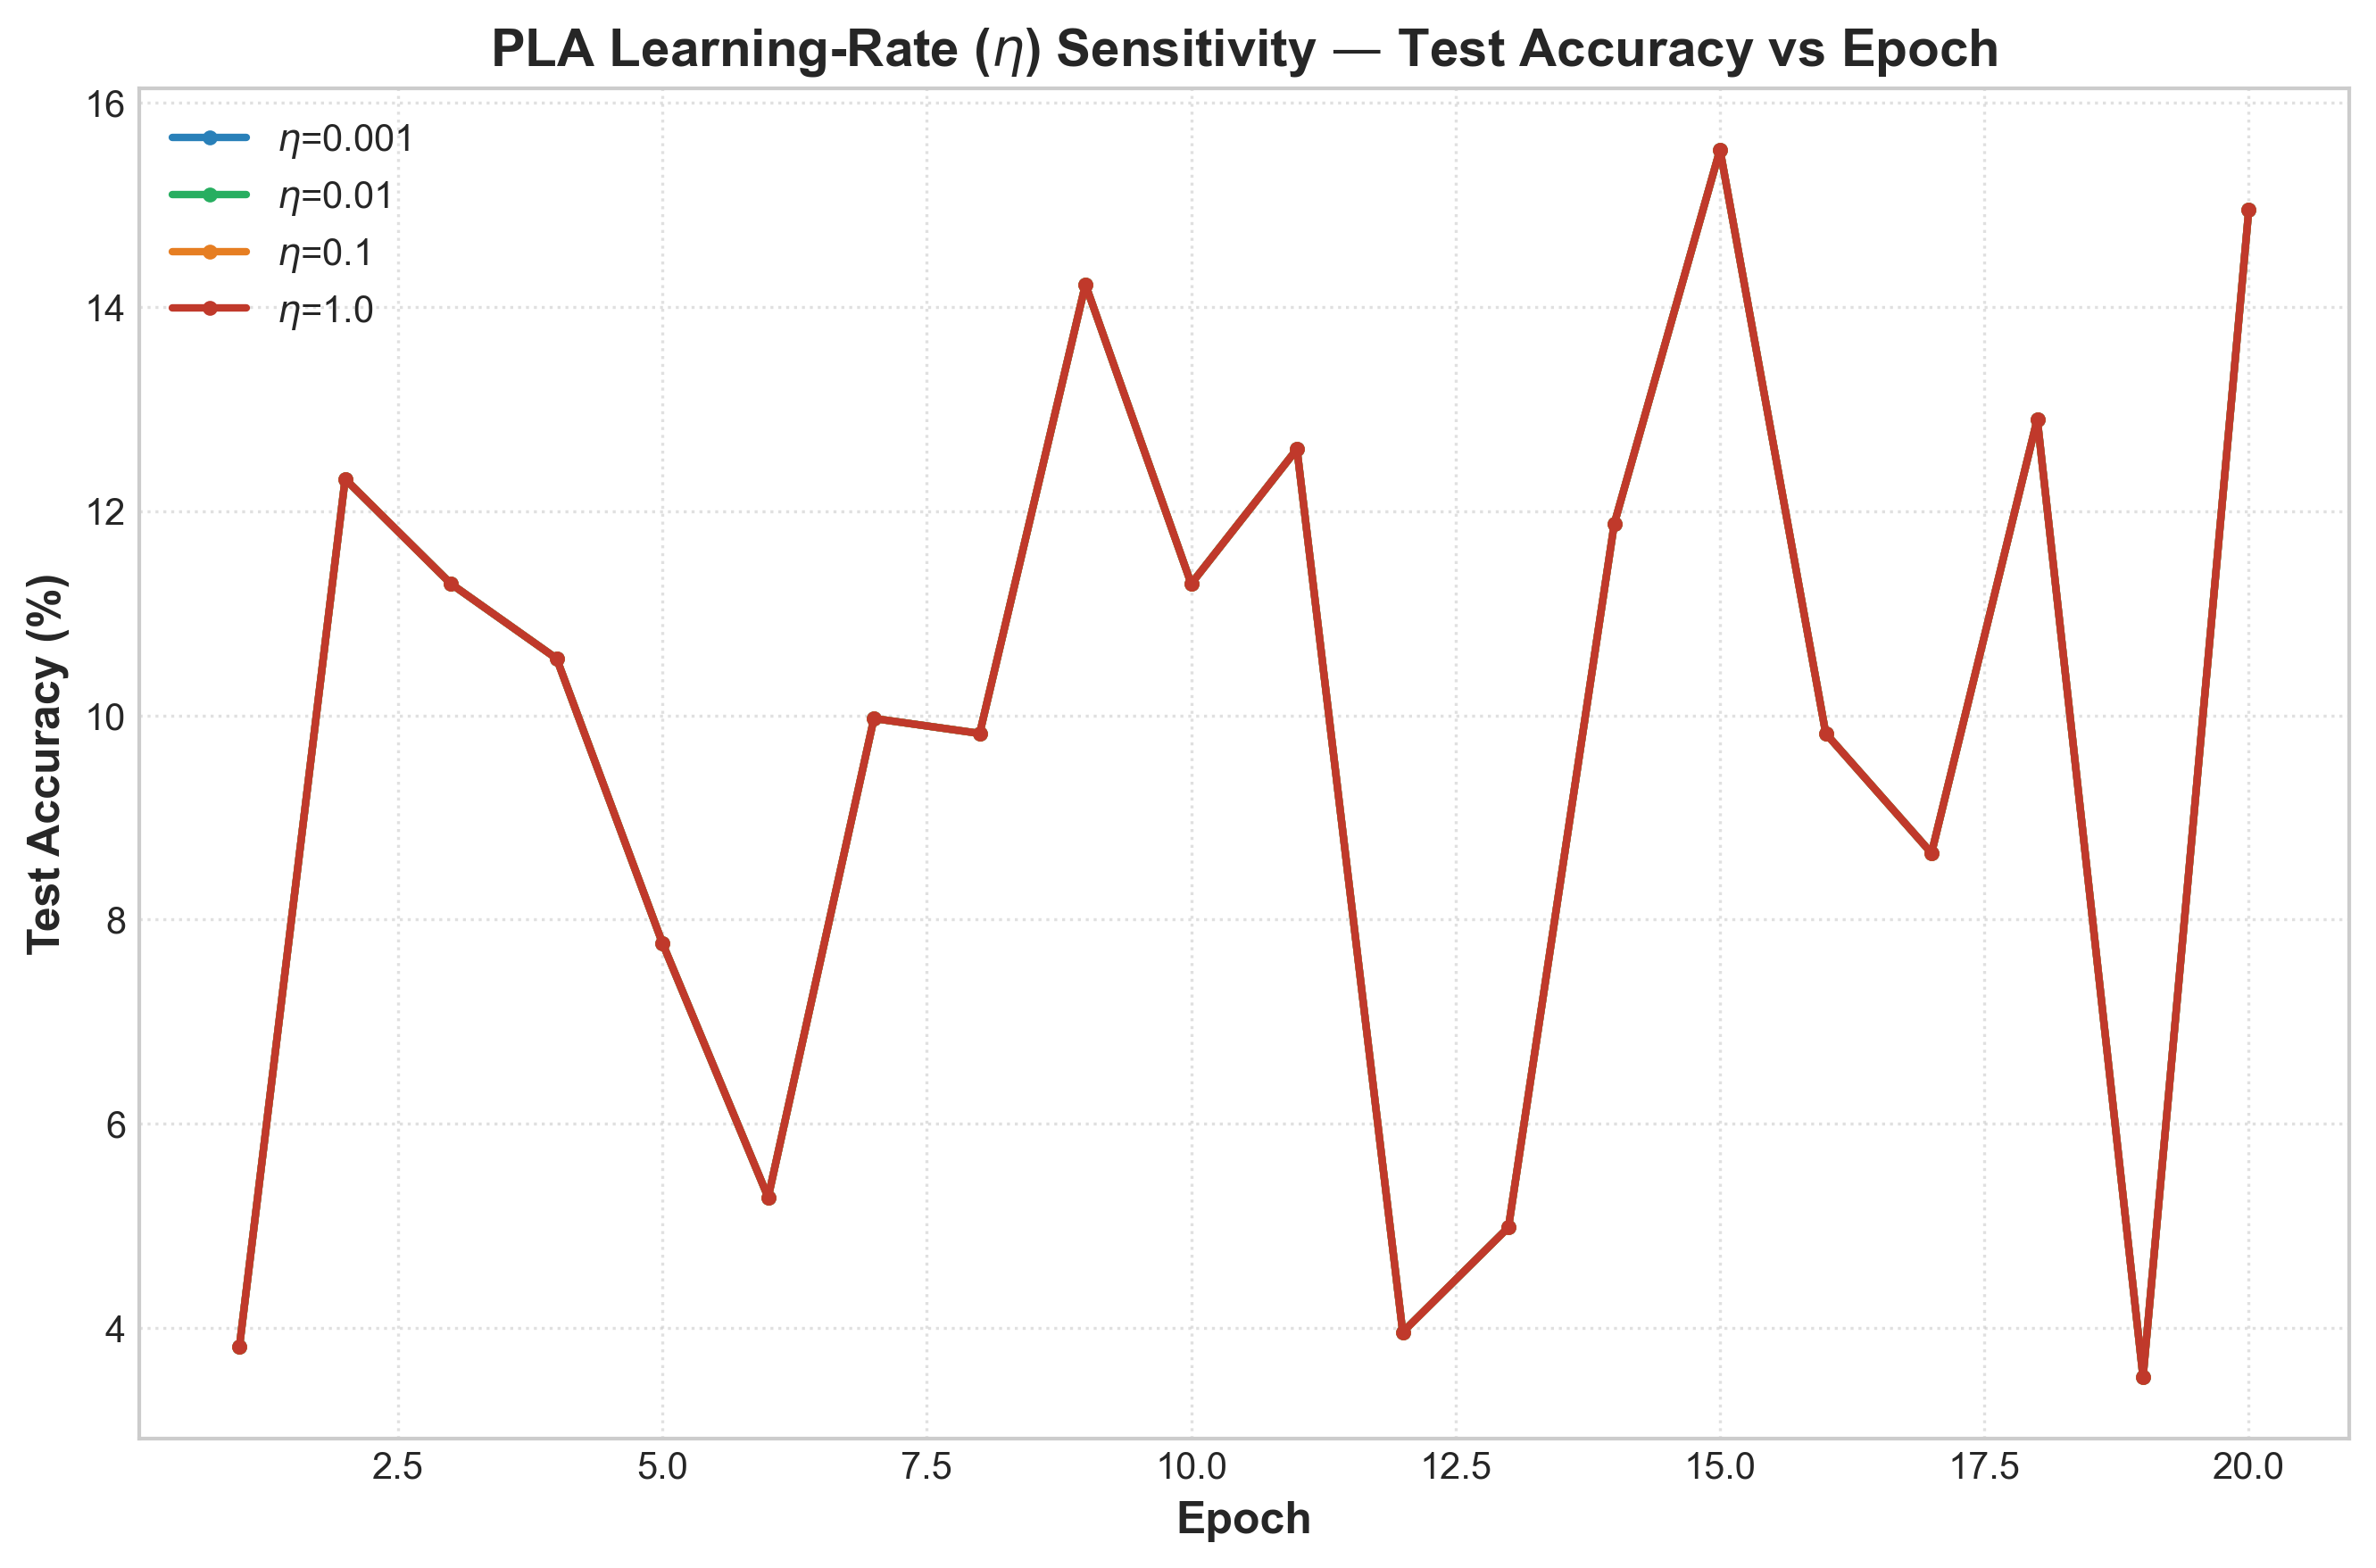
\includegraphics[width=0.85\linewidth]{02_pla_learning_rate_sensitivity.png}
\caption{PLA Learning-Rate Sensitivity — Test Accuracy vs Epoch for $\eta \in \{0.001, 0.01, 0.1, 1.0\}$.}
\end{figure}

\subsection{PLA Final Test Metrics}
\begin{table}[H]
\centering
\caption{PLA Final Test Set Performance}
\begin{tabular}{lc}
\toprule
\textbf{Metric} & \textbf{Value} \\
\midrule
Test Accuracy & \textbf{18.62\%} \\
Precision (macro) & 28.75\% \\
Recall (macro) & 18.62\% \\
F1-Score (macro) & 16.04\% \\
ROC-AUC (micro-avg) & 0.8000 \\
ROC-AUC (macro-avg) & 0.8510 \\
\bottomrule
\end{tabular}
\end{table}

\begin{figure}[H]
\centering
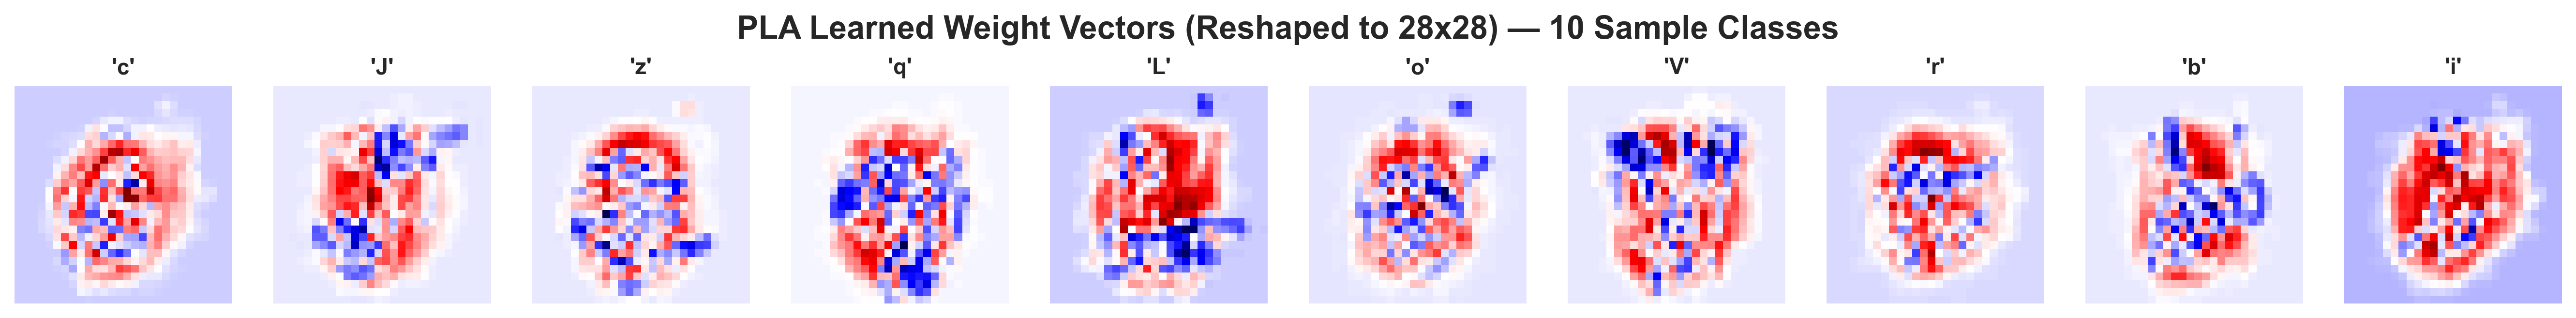
\includegraphics[width=0.85\linewidth]{11_perceptron_weight_visualization.png}
\caption{PLA Learned Weight Vectors, Reshaped to 28$\times$28, for 10 Sample Classes.}
\end{figure}

\section{Model B: MLP Implementation \& Hyperparameter Tuning}
A staged hyperparameter search was used: (1) architecture $\times$ activation, (2) optimizer $\times$ learning rate (using the Stage 1 winner), (3) batch size (using the Stage 1+2 winner) — each evaluated with 3-fold Stratified Cross-Validation via \texttt{GridSearchCV}.

\subsection{Stage 1: Architecture $\times$ Activation Function}
\begin{table}[H]
\centering
\caption{Stage 1 — Architecture x Activation (3-Fold CV Accuracy)}
\label{tab:mlp_stage1}
\begin{tabular}{lccc}
\toprule
\textbf{Hidden Layer Sizes} & \textbf{ReLU} & \textbf{Tanh} & \textbf{Logistic} \\
\midrule
(64,) & 1.54\% (dead) & 16.97\% & 39.04\% \\
\textbf{(128,)} & 1.54\% (dead) & 31.01\% & \textbf{40.18\% (Best)} \\
(128, 64) & 19.24\% (unstable) & 26.10\% & 39.19\% \\
(256, 128, 64) & 1.54\% (dead) & 16.42\% & 31.27\% \\
\bottomrule
\end{tabular}
\end{table}

\noindent
\textbf{Observation:} ReLU catastrophically fails (accuracy $\approx$ chance level, 1.5\%) across almost every architecture — a classic \textbf{dying ReLU} failure mode, caused by normalized $[0,1]$ pixel inputs with a large zero-valued background, small default weight initialization, and a limited 150-iteration training budget, which together drive a large fraction of ReLU units to permanently saturate at zero. \textbf{Logistic (Sigmoid)} activation was the clear winner at every architecture size, and the shallowest single-hidden-layer network \textbf{(128,)} outperformed all deeper architectures.

\begin{figure}[H]
\centering
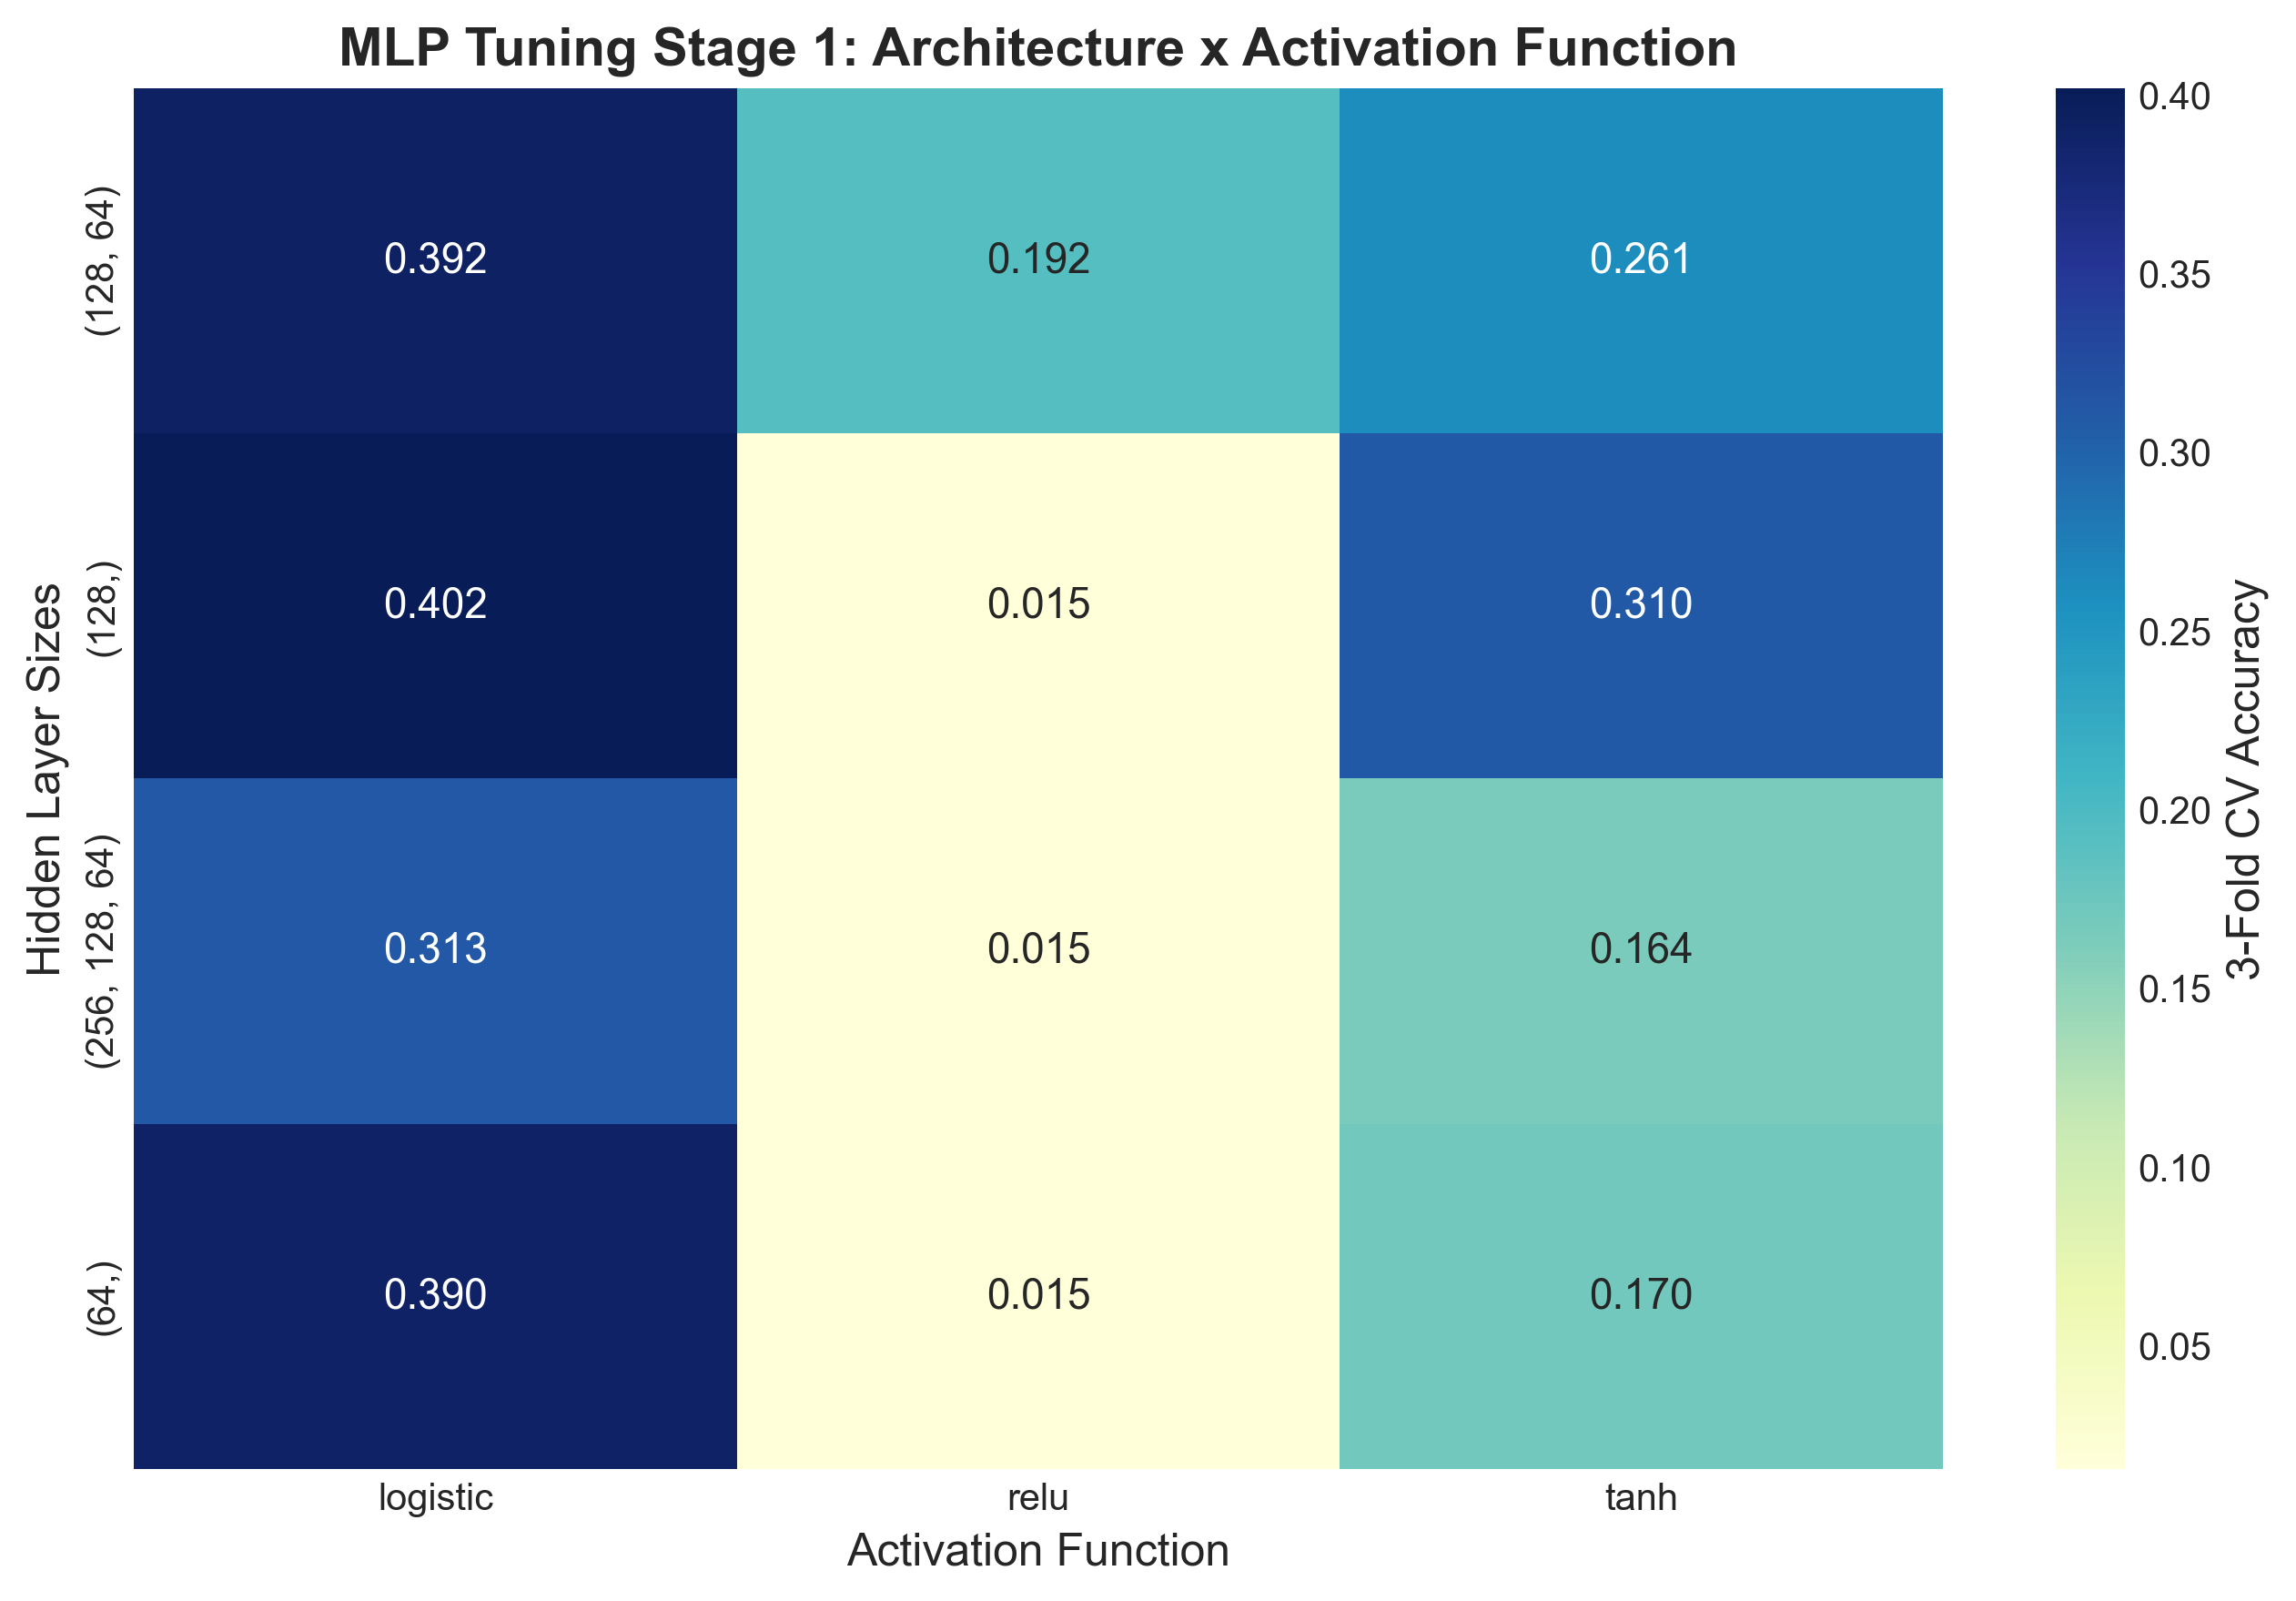
\includegraphics[width=0.75\linewidth]{04_mlp_architecture_activation_tuning.png}
\caption{MLP Tuning Stage 1: Architecture x Activation Function Grid Search Heatmap.}
\end{figure}

\subsection{Stage 2: Optimizer $\times$ Learning Rate}
\begin{table}[H]
\centering
\caption{Stage 2 — Optimizer x Learning Rate (Best Architecture: (128,), Logistic)}
\label{tab:mlp_stage2}
\begin{tabular}{ccc}
\toprule
\textbf{Optimizer} & \textbf{Learning Rate} & \textbf{3-Fold CV Accuracy} \\
\midrule
SGD & 0.0001 & 3.48\% \\
Adam & 0.0001 & 28.12\% \\
SGD & 0.001 & 16.64\% \\
\textbf{Adam} & \textbf{0.001} & \textbf{40.18\% (Best)} \\
SGD & 0.01 & 40.14\% \\
Adam & 0.01 & 1.58\% (diverged) \\
SGD & 0.1 & 22.98\% \\
Adam & 0.1 & 1.58\% (diverged) \\
\bottomrule
\end{tabular}
\end{table}

\noindent
\textbf{Observation:} Adam (lr=0.001) and SGD (lr=0.01) reach nearly identical peak accuracy ($\sim$40\%) through opposite sensitivity profiles — Adam converges well only within a narrow, small learning-rate band and \textbf{diverges catastrophically} at lr $\ge 0.01$, while SGD needs a larger learning rate to make progress within the fixed iteration budget but degrades far more gracefully as lr increases further.

\begin{figure}[H]
\centering
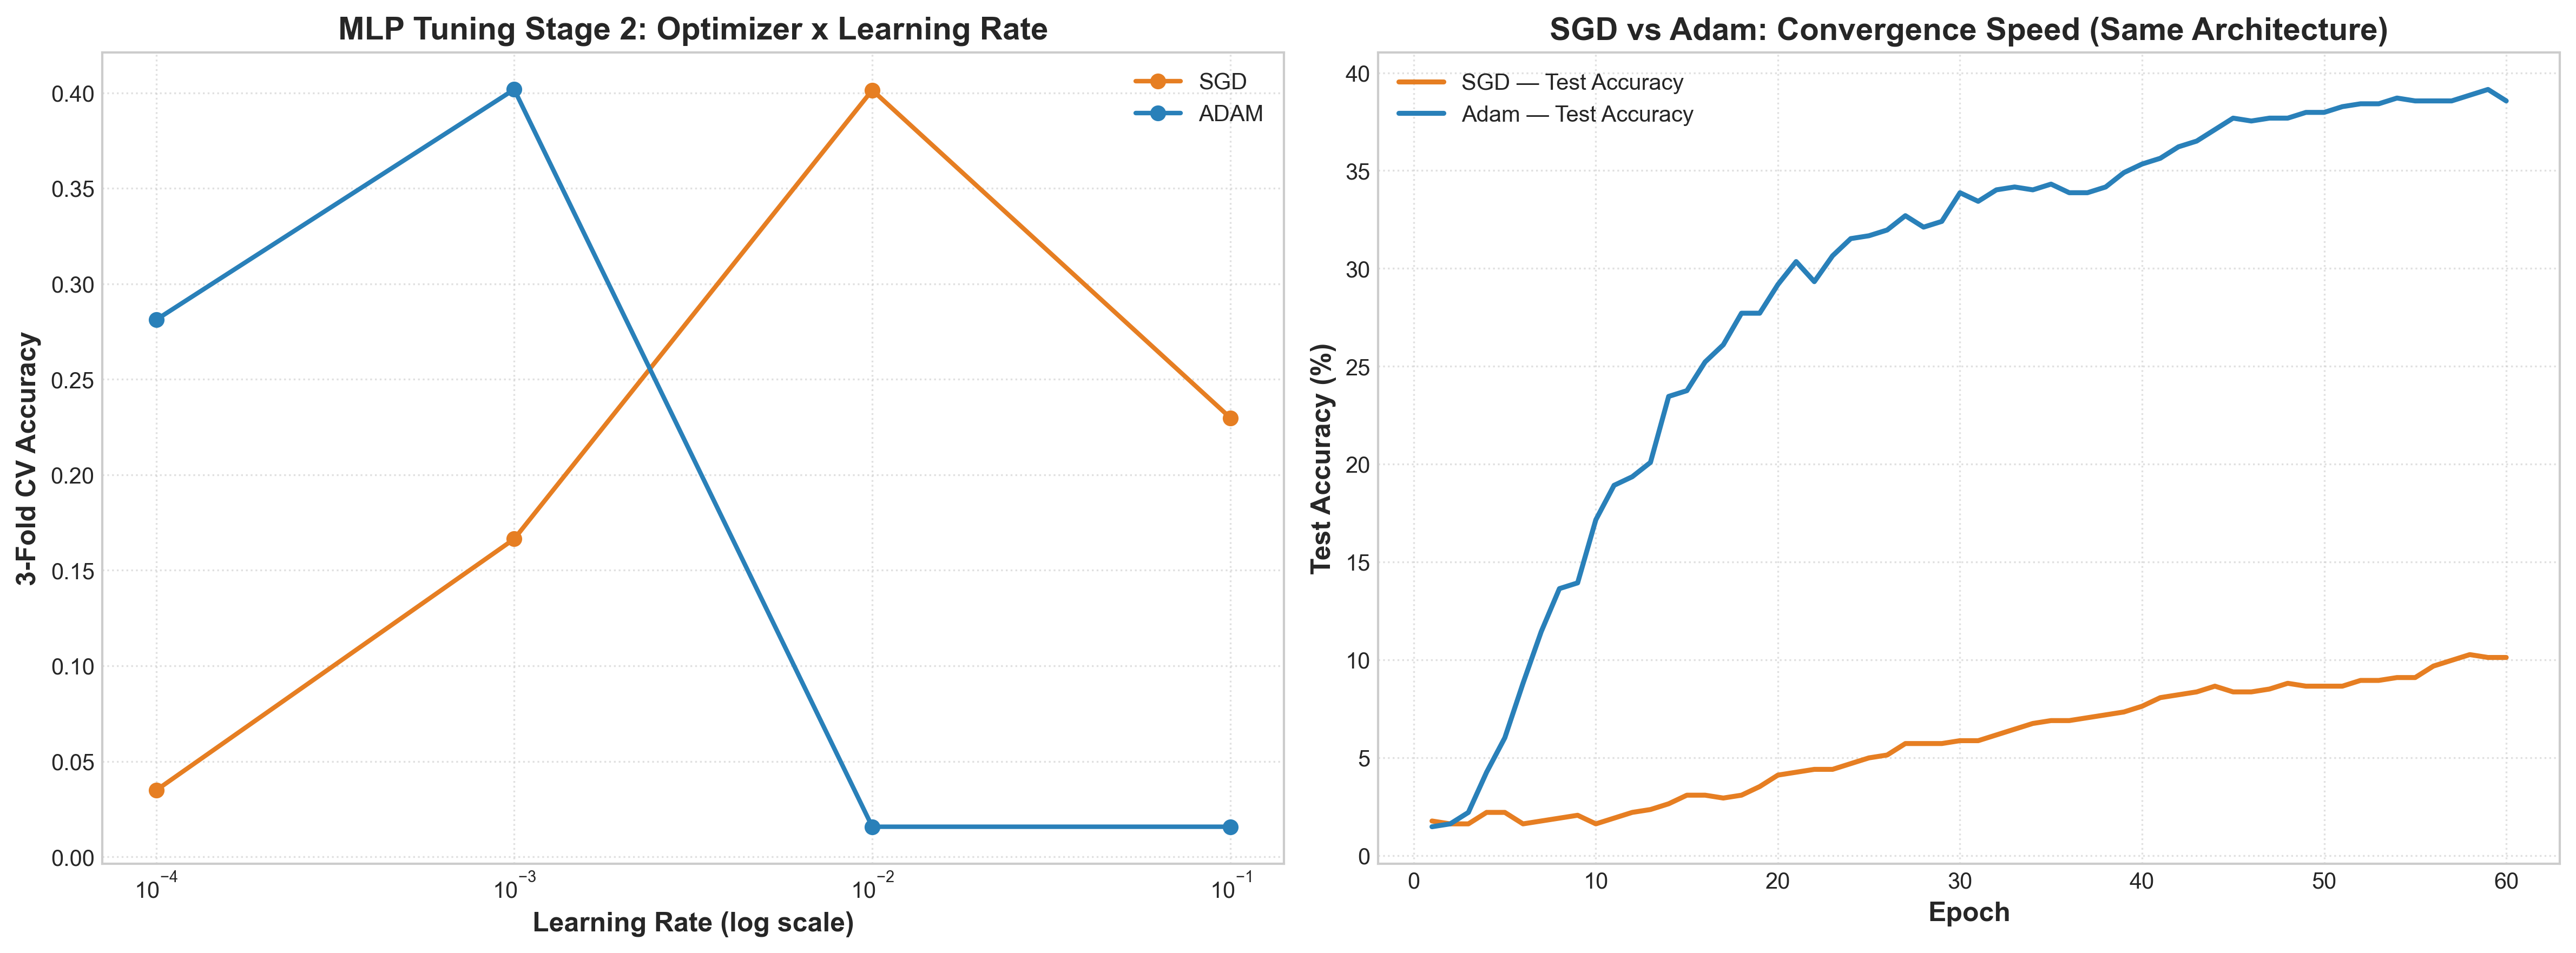
\includegraphics[width=0.98\linewidth]{05_mlp_optimizer_lr_comparison.png}
\caption{Left: Optimizer x Learning-Rate Grid Search. Right: SGD vs Adam Convergence Speed (Same Architecture).}
\end{figure}

\subsection{Stage 3: Batch Size}
\begin{table}[H]
\centering
\caption{Stage 3 — Batch Size (Best Config: (128,), Logistic, Adam, lr=0.001)}
\begin{tabular}{cc}
\toprule
\textbf{Batch Size} & \textbf{3-Fold CV Accuracy} \\
\midrule
16 & 37.50\% \\
32 & 40.18\% \\
\textbf{64} & \textbf{40.87\% (Best)} \\
128 & 39.63\% \\
\bottomrule
\end{tabular}
\end{table}

\begin{figure}[H]
\centering
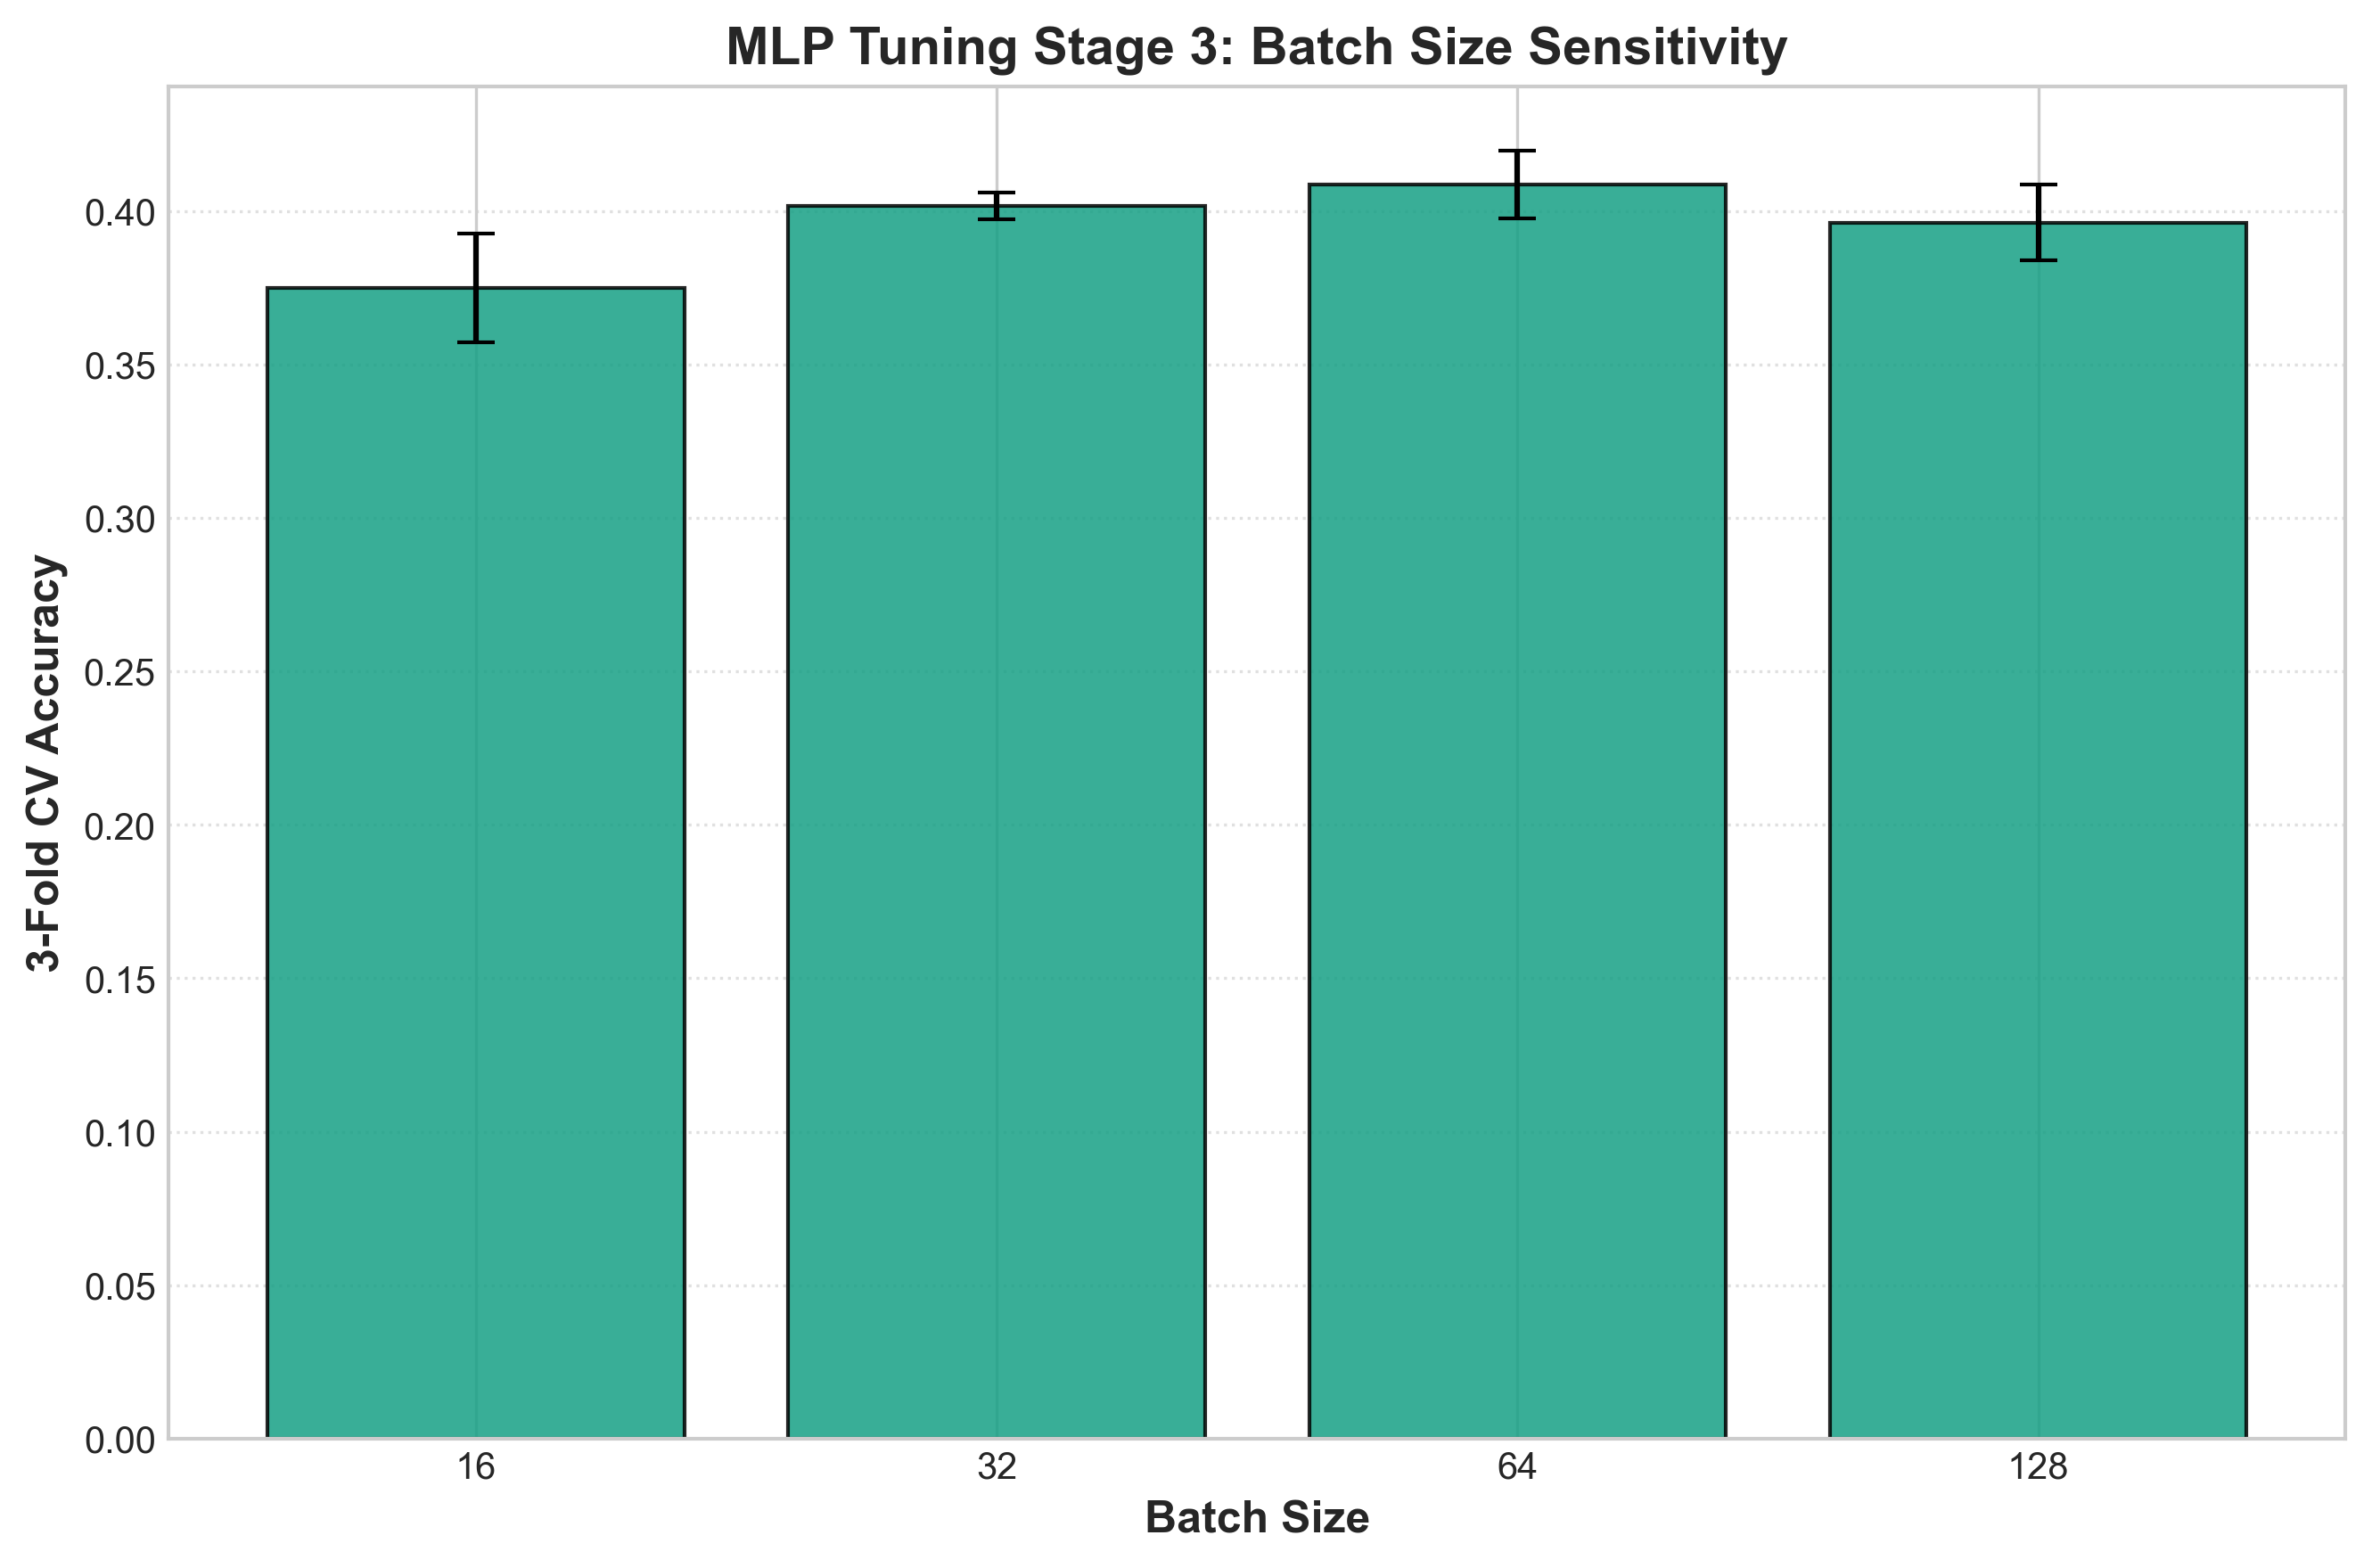
\includegraphics[width=0.75\linewidth]{06_mlp_batch_size_comparison.png}
\caption{MLP Tuning Stage 3: Batch Size Sensitivity.}
\end{figure}

\subsection{Final Chosen MLP Configuration}
\begin{table}[H]
\centering
\caption{Final MLP Hyperparameters and Justification}
\label{tab:mlp_final_config}
\resizebox{\linewidth}{!}{
\begin{tabular}{lll}
\toprule
\textbf{Hyperparameter} & \textbf{Selected Value} & \textbf{Justification} \\
\midrule
Architecture & (128,) — single hidden layer & Outperformed deeper nets; small $\sim$44 samples/class cannot support more parameters \\
Activation & Logistic (Sigmoid) & Only activation avoiding the dying-unit failure on this input distribution \\
Cost Function & Cross-Entropy (log-loss) & Standard for softmax multiclass classification \\
Optimizer & Adam & Best CV accuracy at its optimal learning rate \\
Learning Rate & 0.001 & Best Adam configuration; avoided divergence seen at lr $\ge 0.01$ \\
Batch Size & 64 & Best 3-fold CV accuracy; balances gradient noise vs convergence speed \\
\bottomrule
\end{tabular}
}
\end{table}

\subsection{MLP Final Test Metrics}
\begin{table}[H]
\centering
\caption{MLP Final Test Set Performance}
\begin{tabular}{lc}
\toprule
\textbf{Metric} & \textbf{Value} \\
\midrule
Test Accuracy & \textbf{38.56\%} \\
Precision (macro) & 42.02\% \\
Recall (macro) & 38.56\% \\
F1-Score (macro) & 37.93\% \\
ROC-AUC (micro-avg) & 0.9069 \\
ROC-AUC (macro-avg) & 0.9037 \\
\bottomrule
\end{tabular}
\end{table}

\section{A/B Comparison: PLA vs Tuned MLP}
\begin{table}[H]
\centering
\caption{A/B Comparison Summary}
\label{tab:ab_comparison}
\resizebox{\linewidth}{!}{
\begin{tabular}{lccc}
\toprule
\textbf{Metric} & \textbf{PLA (Model A)} & \textbf{MLP -- Tuned (Model B)} & \textbf{Improvement} \\
\midrule
Test Accuracy & 18.62\% & \textbf{38.56\%} & \textbf{+19.94 pp (2.07x)} \\
Precision (macro) & 28.75\% & \textbf{42.02\%} & +13.27 pp \\
Recall (macro) & 18.62\% & \textbf{38.56\%} & +19.94 pp \\
F1-Score (macro) & 16.04\% & \textbf{37.93\%} & \textbf{+21.89 pp (2.36x)} \\
ROC-AUC (micro-avg) & 0.8000 & \textbf{0.9069} & +0.1069 \\
ROC-AUC (macro-avg) & 0.8510 & \textbf{0.9037} & +0.0527 \\
Training Convergence & Oscillates, never stabilizes & Smooth, monotonic improvement & MLP converges; PLA does not \\
\bottomrule
\end{tabular}
}
\end{table}

\begin{figure}[H]
\centering
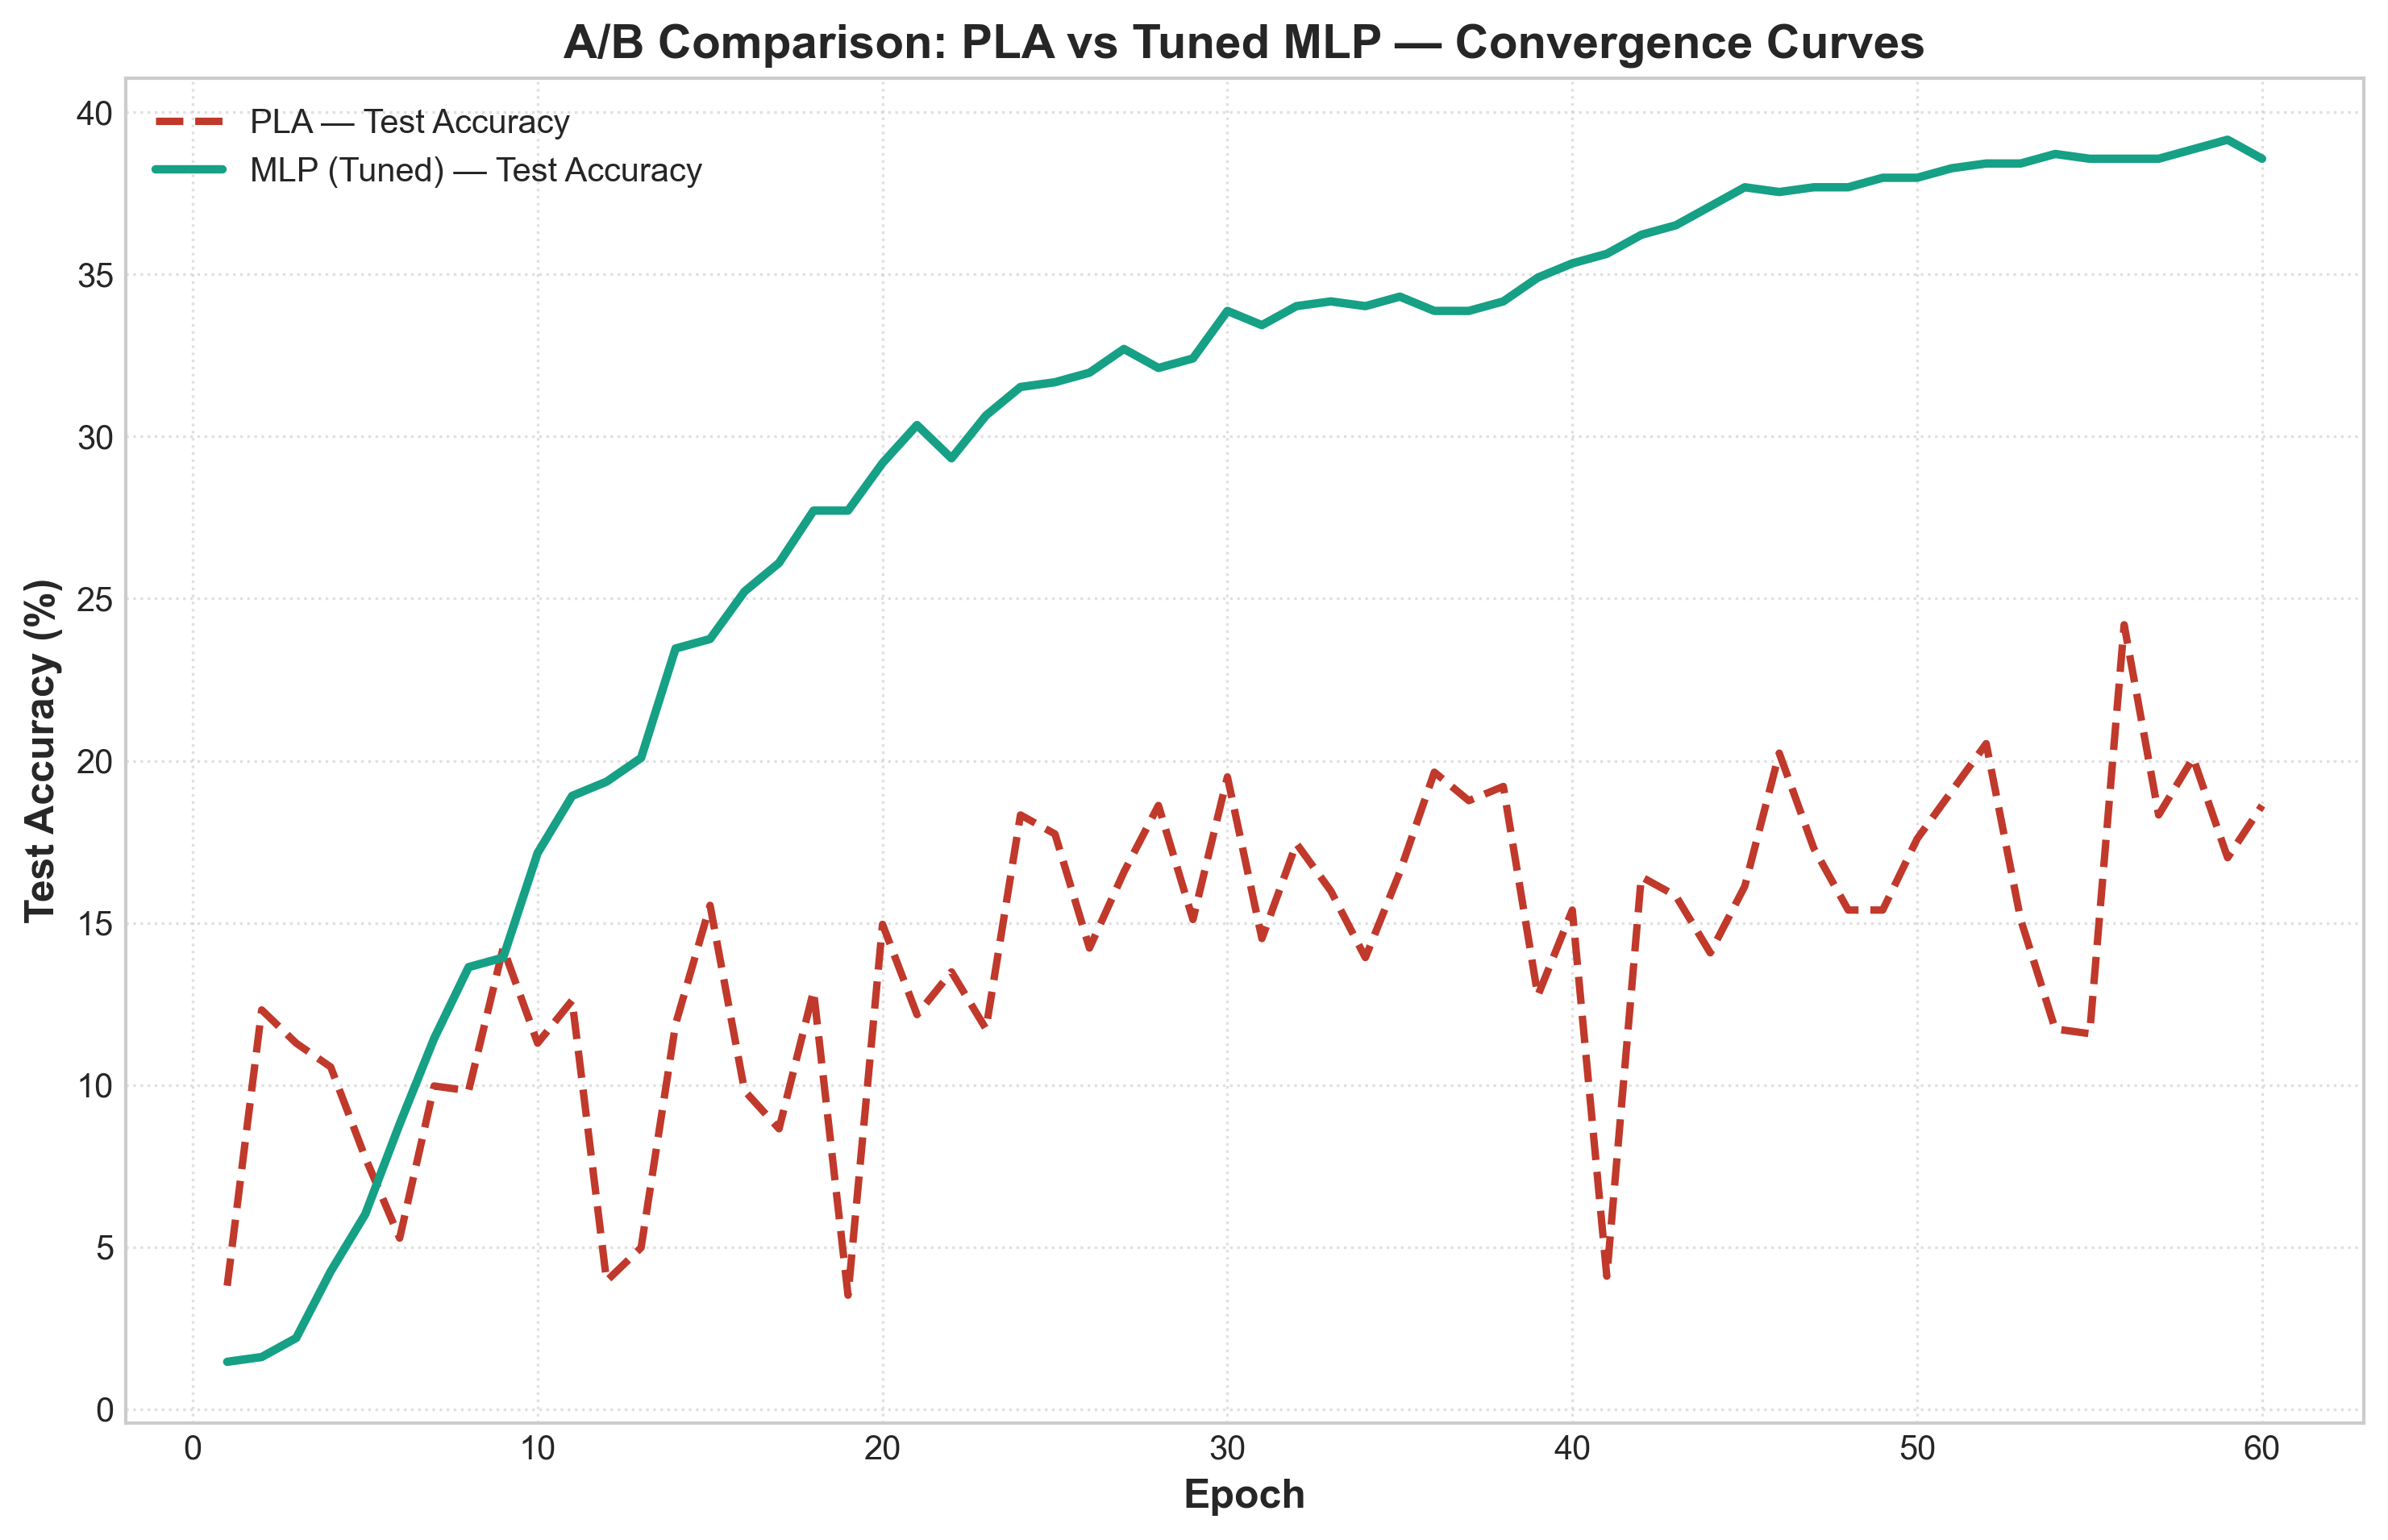
\includegraphics[width=0.85\linewidth]{07_pla_vs_mlp_convergence_curves.png}
\caption{A/B Comparison: PLA vs Tuned MLP — Test Accuracy Convergence Curves.}
\end{figure}

\begin{figure}[H]
\centering
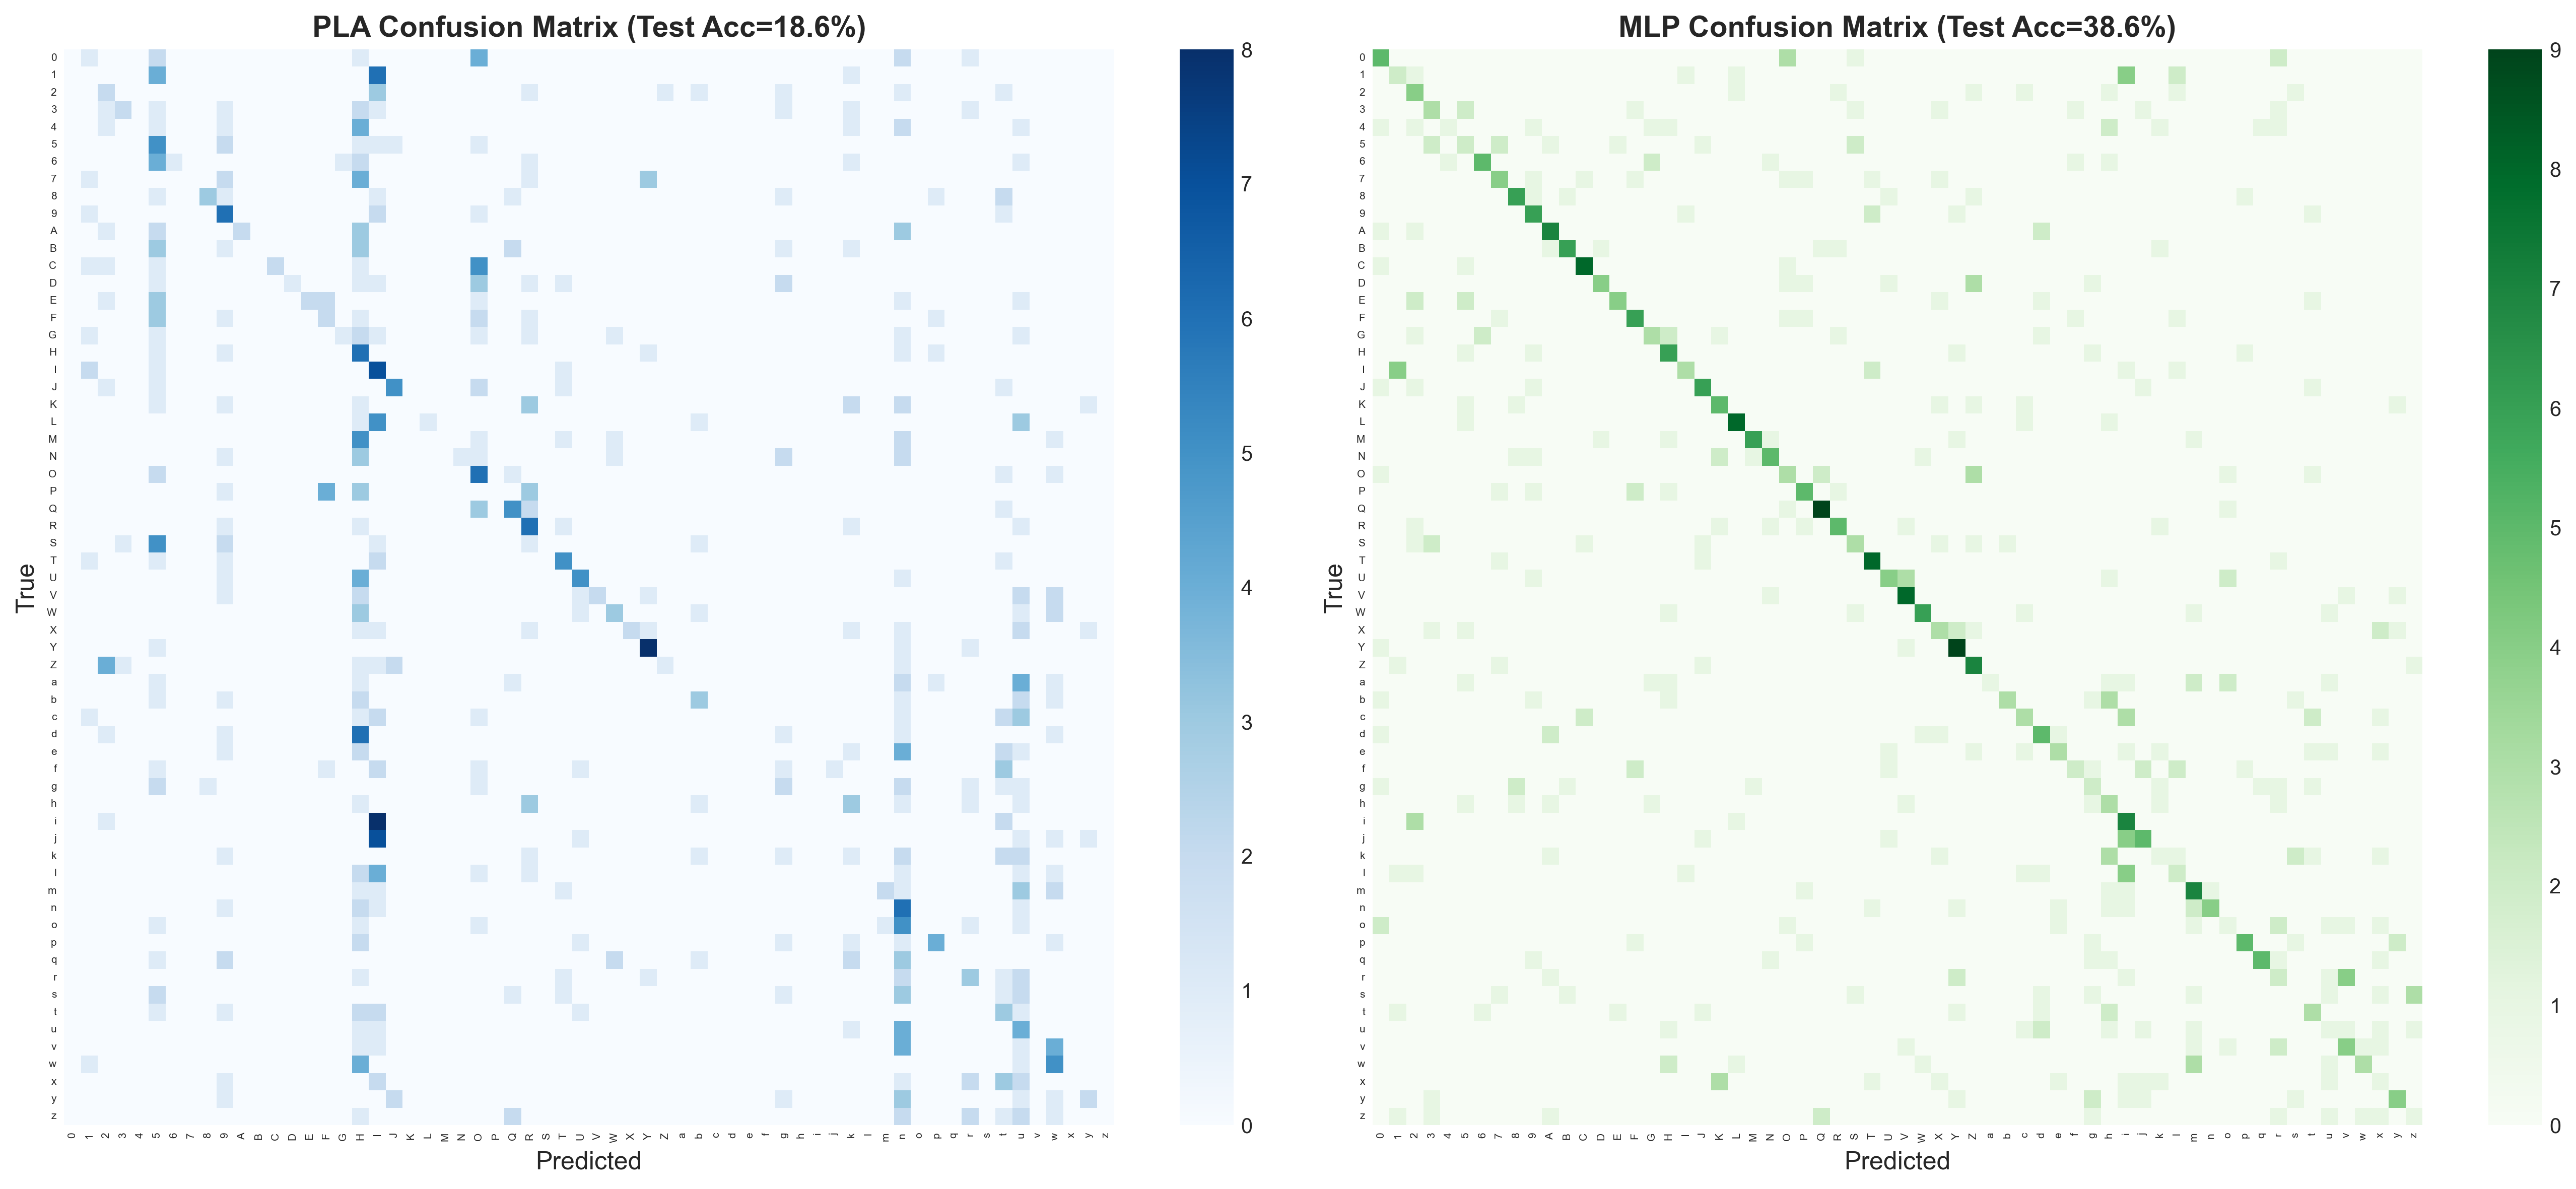
\includegraphics[width=0.98\linewidth]{08_confusion_matrices_pla_vs_mlp.png}
\caption{Confusion Matrices (62x62, Test Set): PLA (Left) vs MLP (Right).}
\end{figure}

\begin{figure}[H]
\centering
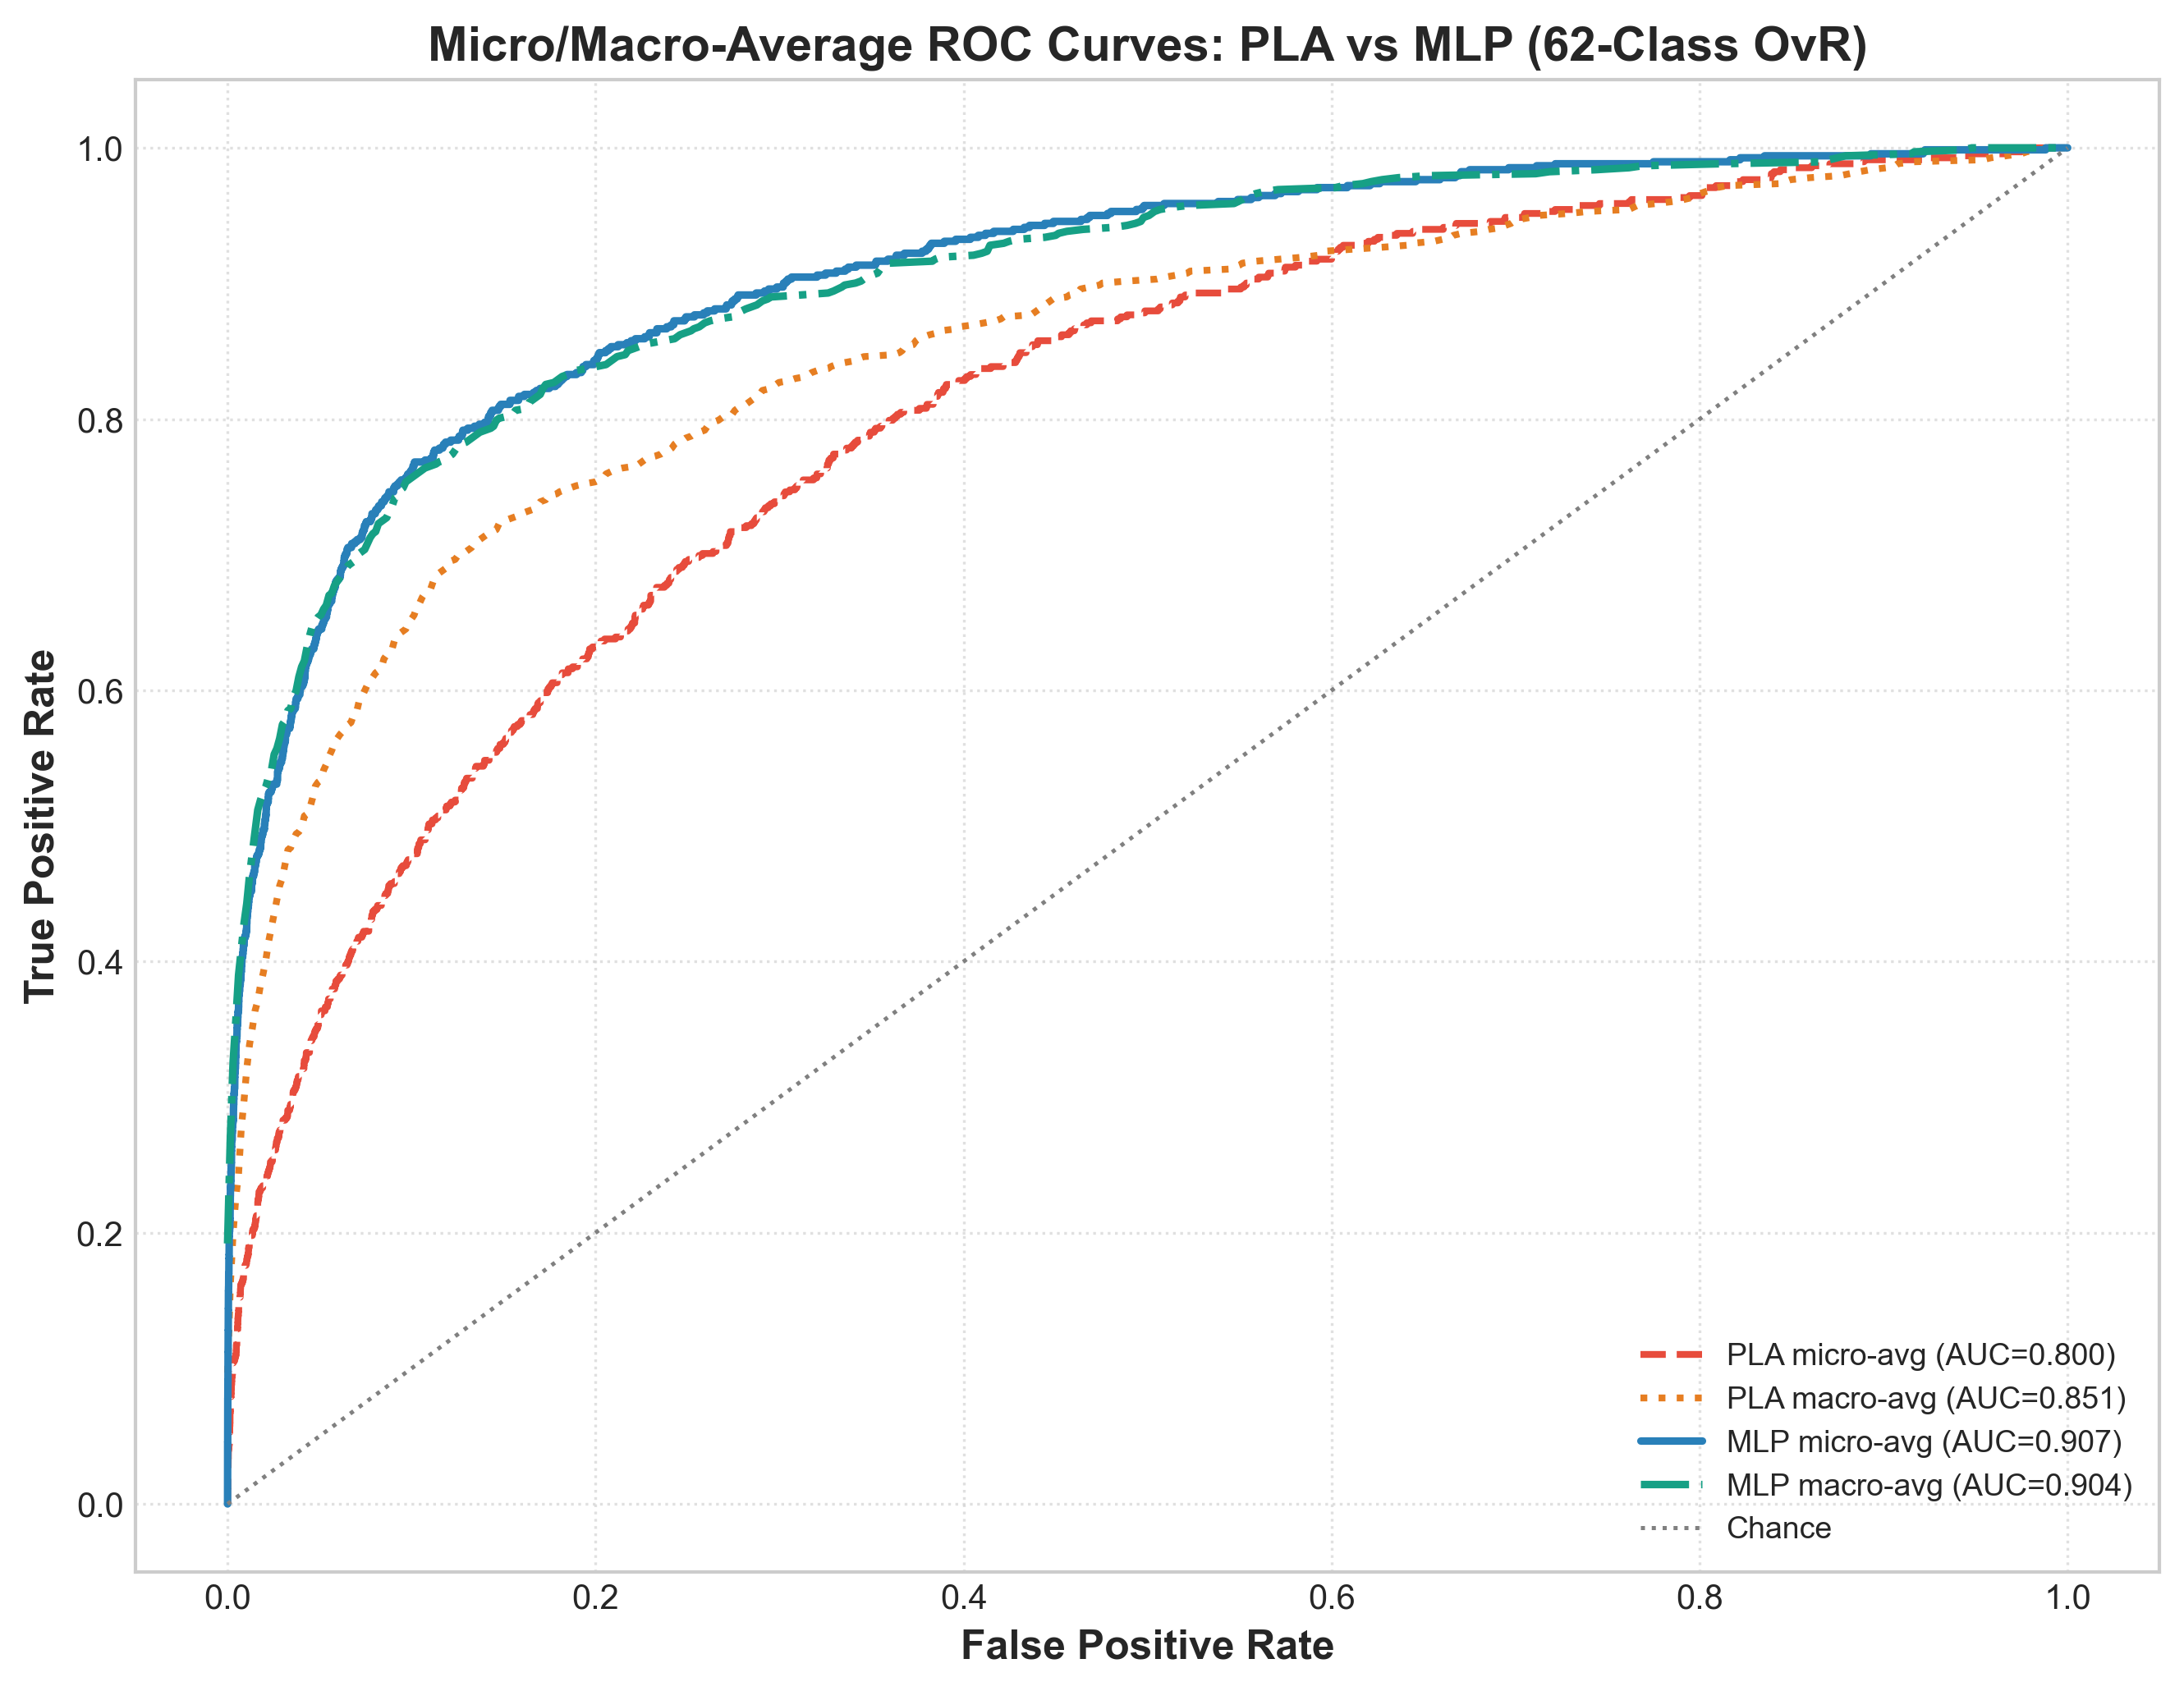
\includegraphics[width=0.85\linewidth]{09_roc_curves_micro_macro.png}
\caption{Micro/Macro-Average ROC Curves: PLA vs MLP (62-Class One-vs-Rest).}
\end{figure}

\begin{figure}[H]
\centering
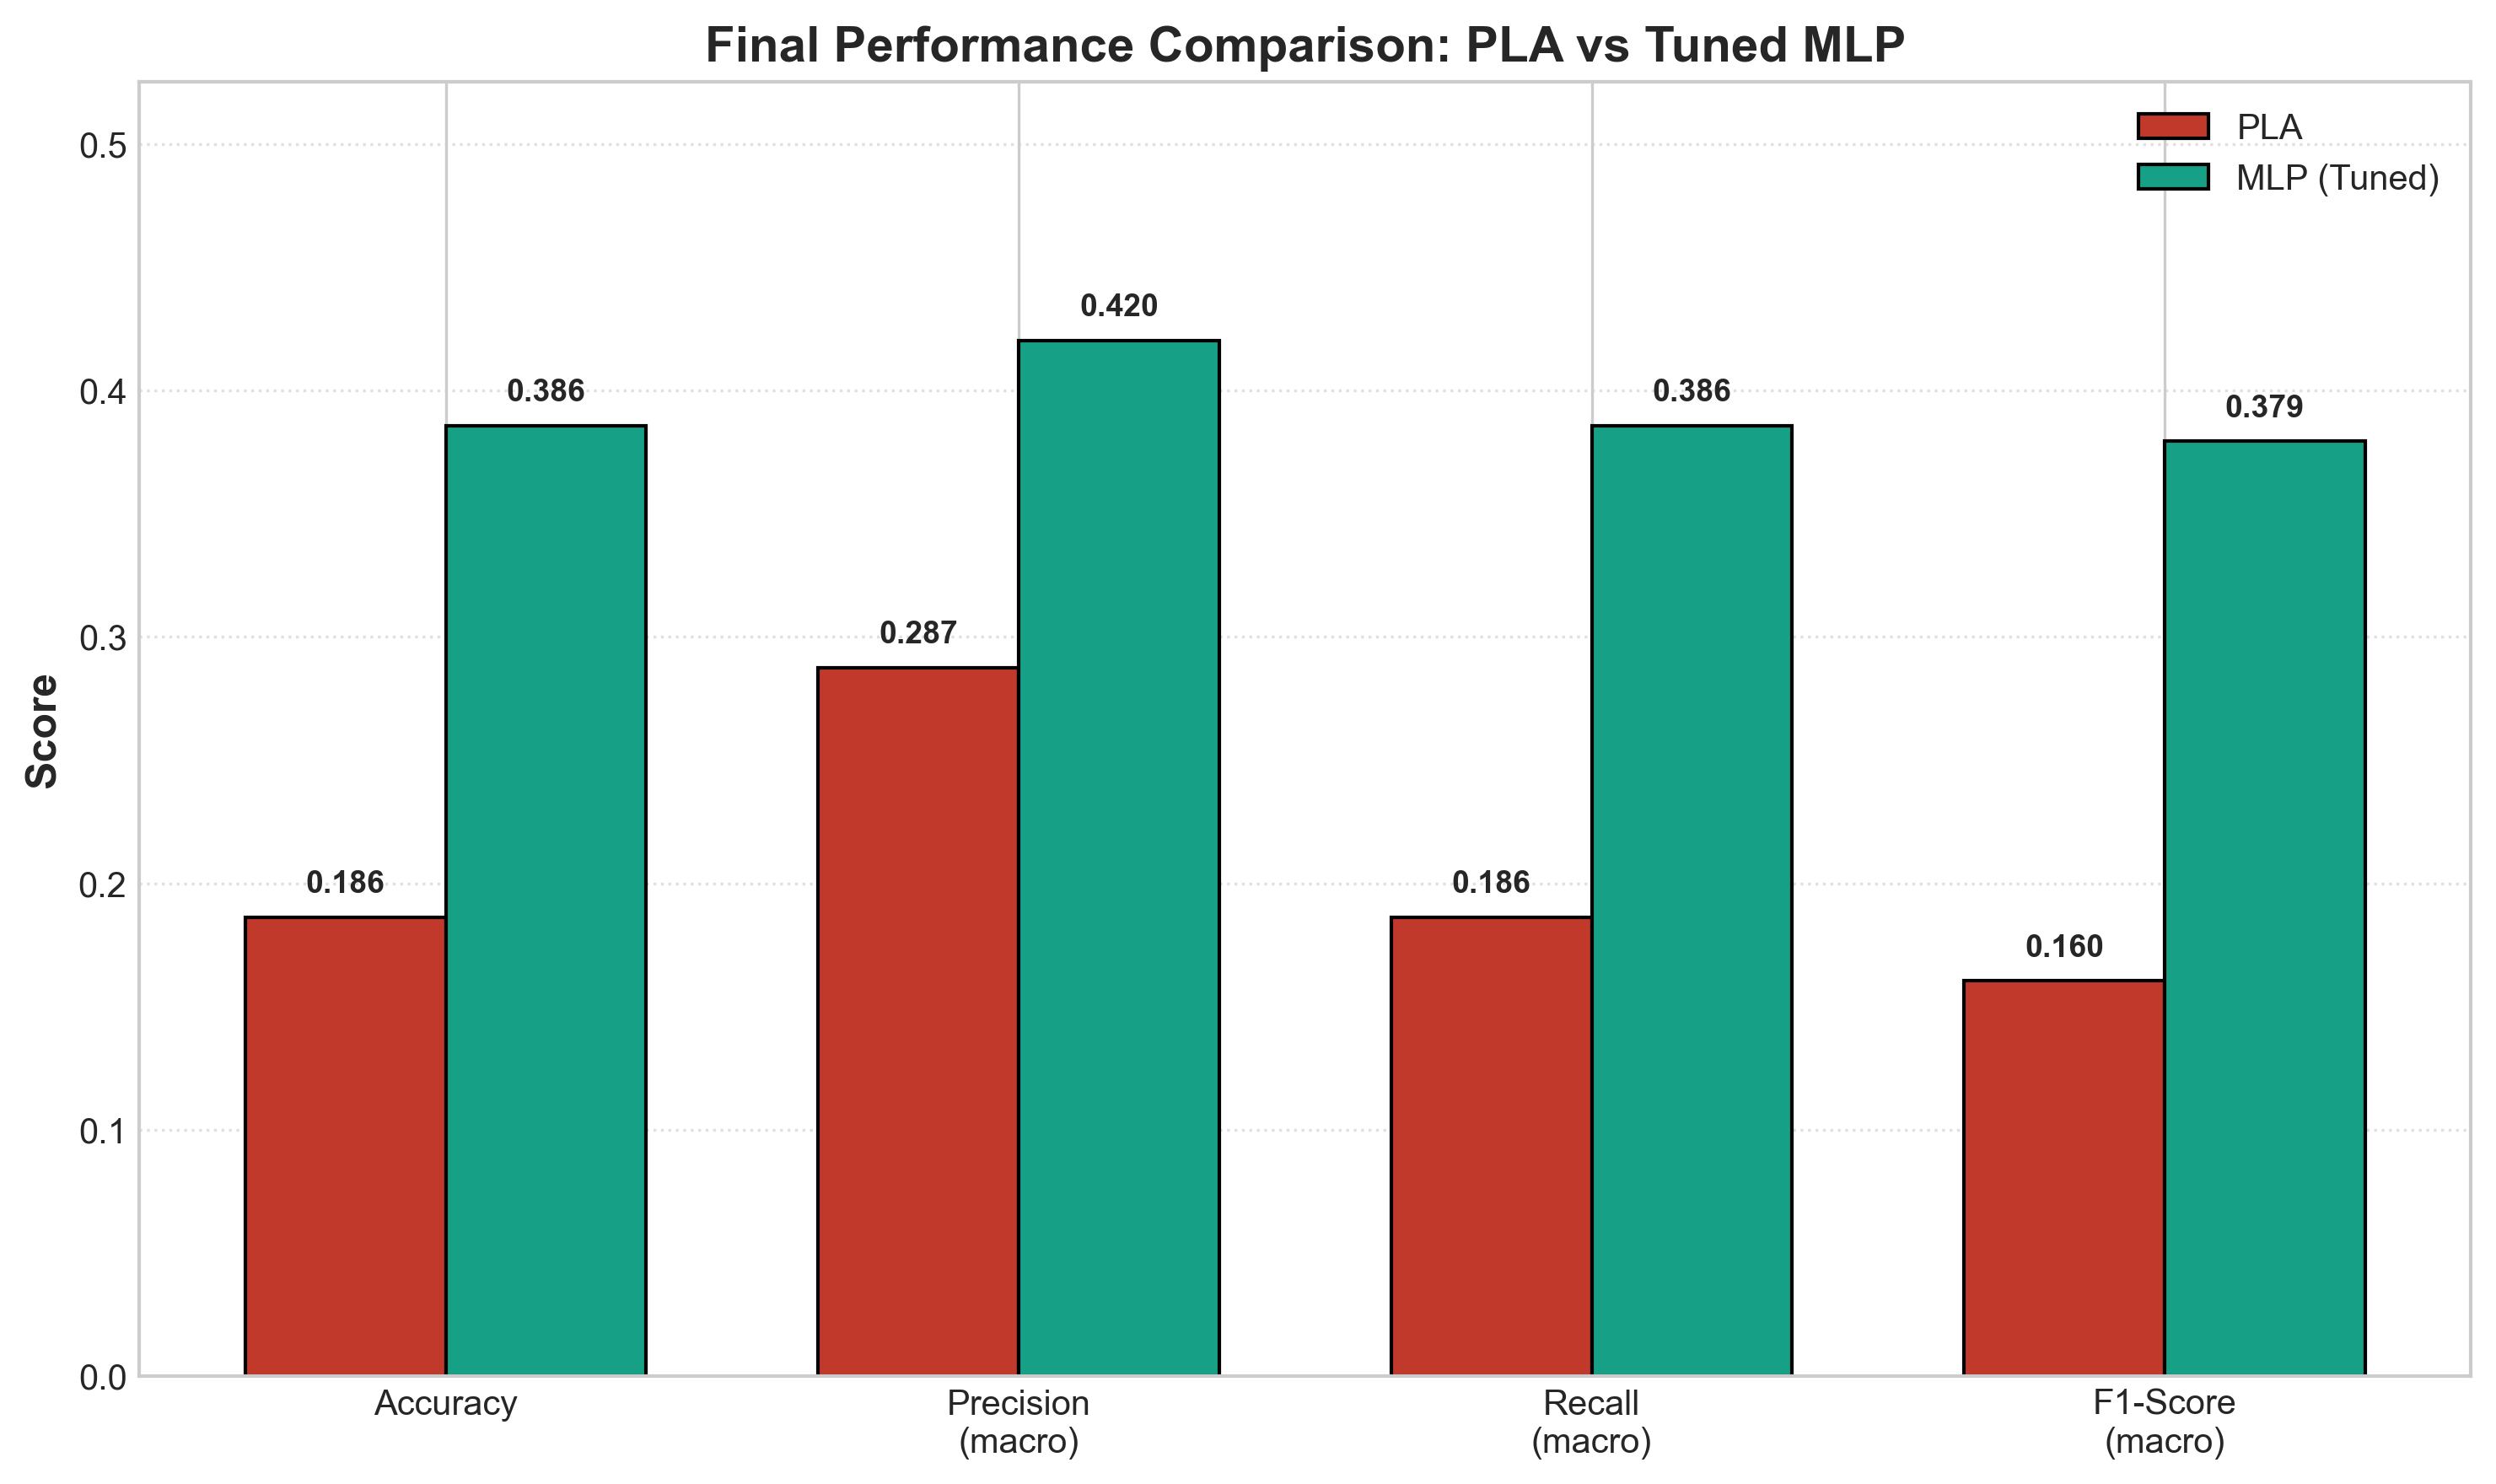
\includegraphics[width=0.85\linewidth]{10_performance_metrics_comparison.png}
\caption{Final Performance Comparison: Accuracy, Precision, Recall, and F1-Score (macro) — PLA vs Tuned MLP.}
\end{figure}

\section{Answers to Observation Questions \& Detailed Discussion}

\subsection{1. Why does PLA underperform compared to MLP?}
PLA is a strictly linear classifier — each of its 62 One-vs-Rest sub-perceptrons can only carve the 784-dimensional pixel space with a single hyperplane. Handwritten character classes are not linearly separable: character pairs such as '0'/'O' or 'l'/'I'/'1' differ by subtle, non-linear stroke variations that no single hyperplane can cleanly separate from the other 61 classes simultaneously. This is directly visible in the training convergence curve (Figure~\ref{fig:pla_conv}): rather than settling, PLA's misclassification count and accuracy oscillate indefinitely across all 60 epochs, and its confusion matrix shows predictions collapsing onto a handful of "attractor" columns rather than a clean diagonal. MLP, by contrast, learns a non-linear decision boundary through its hidden layer, sigmoid activation, backpropagation, and the Adam optimizer — achieving a clean diagonal-dominant confusion matrix at roughly double PLA's accuracy.

\subsection{2. Which hyperparameters had the most impact on MLP performance?}
\textbf{Activation function} had the largest impact by far: switching ReLU $\to$ Logistic changed CV accuracy from $\sim$1.5\% (chance level) to $\sim$40\% at the same architecture. \textbf{Learning rate} was second, specifically its interaction with optimizer choice — Adam collapsed from 40.18\% to 1.58\% with just a 10x lr increase. \textbf{Architecture depth} had a clear but smaller effect: deeper networks consistently underperformed the single-layer (128,) network by 5--10 percentage points, since $\sim$44 training images/class cannot support additional parameters. \textbf{Batch size} had the smallest impact, varying CV accuracy by only $\sim$3.4 percentage points.

\subsection{3. Did optimizer choice (SGD vs Adam) affect convergence?}
Yes, substantially. At their respective optimal learning rates, SGD (lr=0.01, 40.14\%) and Adam (lr=0.001, 40.18\%) achieved nearly identical peak accuracy, but Adam required a 10x smaller learning rate and diverged catastrophically (to $\sim$1.6\%, chance level) at lr $\ge 0.01$, because its adaptive per-parameter scaling amplifies effective step sizes once gradients shrink near convergence. SGD, lacking this amplification, degraded far more gracefully as learning rate increased (22.98\% even at lr=0.1) — demonstrating that Adam's fast, low-lr convergence advantage comes with a narrower stable learning-rate range than plain SGD.

\subsection{4. Did adding more hidden layers always improve results? Why or why not?}
No — deeper was consistently worse. With Logistic activation, CV accuracy fell monotonically with depth: (128,) $\to$ 40.18\%, (128,64) $\to$ 39.19\%, (256,128,64) $\to$ 31.27\%; the same pattern held for Tanh. This reflects the classic bias-variance trade-off: with only $\sim$44 training images per class, deeper/wider networks add far more trainable parameters than the data can support, causing them to overfit training folds and generalize worse. A single, moderately-sized hidden layer was the capacity sweet spot for this dataset's scale.

\subsection{5. Did MLP show overfitting? How could it be mitigated?}
To a degree, yes — declining cross-validated (not just training) accuracy as network depth increases is itself an overfitting signature, and the final model's test-accuracy convergence curve shows a narrowing but persistent train-test gap as epochs increase. This could be further mitigated by: (a) L2 weight regularization (\texttt{alpha} in \texttt{MLPClassifier}) to penalize large weights, (b) \texttt{early\_stopping=True} with a held-out validation split, (c) data augmentation (small rotations/translations/elastic distortions) to synthetically enlarge the $\sim$44-sample-per-class training set, and (d) dropout-style regularization if migrating to a deep-learning framework such as PyTorch or TensorFlow.

\section{Conclusion}
This experiment provides a clear, quantitatively grounded A/B comparison between a linear (PLA) and non-linear (MLP) classifier on a genuinely hard, small-sample, 62-class handwritten-character recognition task:
\begin{enumerate}
\item PLA's step-activation, hyperplane-only decision boundaries cannot separate the character classes, and its training never converges (accuracy oscillating around 15--20\% for the entire 60-epoch run).
\item Systematic staged hyperparameter tuning — architecture/activation, then optimizer/learning-rate, then batch size — allowed the MLP to more than double PLA's test accuracy (\textbf{18.62\% $\to$ 38.56\%}) and macro-F1 score (\textbf{16.04\% $\to$ 37.93\%}), with a substantially higher and smoothly-converging ROC-AUC (0.80 $\to$ 0.91 micro-average).
\item The tuning process surfaced two important, non-obvious findings: \textbf{ReLU activation catastrophically fails} ("dies") on this small, sparse, $[0,1]$-normalized dataset while Logistic activation thrives, and \textbf{deeper architectures consistently underperform} a single hidden layer given the limited $\sim$44-samples-per-class training budget.
\item Both findings underscore that matching model capacity and activation choice to dataset scale and structure is as important as the headline choice between a linear and non-linear model.
\end{enumerate}

\end{document}
